% Capitolul 12: Modele de scoring
% Statistica piețelor financiare -- Program de licență, Academia de Studii Economice din București
% GENERAT de latex/build_chapter12.py -- modificați generatorul, nu acest fișier.

\newcommand{\coursename}{Statistica piețelor financiare}
\def\sfmlang{ro}
% Preambul comun SFM -- Statistica piețelor financiare / Statistics of Financial Markets (Beamer, 16:9)
% Același design ca MFM. Înainte de % Preambul comun SFM -- Statistica piețelor financiare / Statistics of Financial Markets (Beamer, 16:9)
% Același design ca MFM. Înainte de % Preambul comun SFM -- Statistica piețelor financiare / Statistics of Financial Markets (Beamer, 16:9)
% Același design ca MFM. Înainte de \input{../../latex/preamble} se definește
%   \newcommand{\coursename}{Statistics of Financial Markets}      (EN)
%   \newcommand{\coursename}{Statistica piețelor financiare}       (RO)  și  \def\sfmlang{ro}
% Fișierele .tex se află în EN/Courses, EN/Seminars, RO/Cursuri, RO/Seminarii (două niveluri sub rădăcină).
% Deck-urile sînt generate de latex/build_chapterN.py / build_seminarN.py (vezi latex/sfm_build.py).

\documentclass[9pt, aspectratio=169, t]{beamer}
\providecommand{\coursename}{Statistics of Financial Markets}

% Ensure content fits on slides
\setbeamersize{text margin left=8mm, text margin right=8mm}

%=============================================================================
% THEME AND STYLE CONFIGURATION
%=============================================================================
\usetheme{default}
% Using default theme for clean header/footer control

% Color Palette (matching Redispatch PDF)
\definecolor{MainBlue}{RGB}{26, 58, 110}
\definecolor{AccentBlue}{RGB}{26, 58, 110}
\definecolor{IDAred}{RGB}{205, 0, 0}
\definecolor{DarkGray}{RGB}{51, 51, 51}
\definecolor{MediumGray}{RGB}{128, 128, 128}
\definecolor{LightGray}{RGB}{248, 248, 248}
\definecolor{VeryLightGray}{RGB}{235, 235, 235}
\definecolor{KeynoteGray}{RGB}{218, 218, 218}
\definecolor{SectionGray}{RGB}{120, 120, 120}
\definecolor{FooterGray}{RGB}{100, 100, 100}
\definecolor{Crimson}{RGB}{220, 53, 69}
\definecolor{Forest}{RGB}{46, 125, 50}
\definecolor{Amber}{RGB}{181, 133, 63}
\definecolor{Orange}{RGB}{230, 126, 34}
\definecolor{Purple}{RGB}{142, 68, 173}

% Gradient background (exact Keynote 315° gradient: white to RGB 218,218,218)
\setbeamertemplate{background}{%
    \begin{tikzpicture}[remember picture, overlay]
        \shade[shading=axis, shading angle=315,
        top color=white, bottom color=KeynoteGray]
        (current page.south west) rectangle (current page.north east);
    \end{tikzpicture}%
}
% Fallback solid color for compatibility
\setbeamercolor{background canvas}{bg=}

\setbeamercolor{palette primary}{bg=MainBlue, fg=white}
\setbeamercolor{palette secondary}{bg=MainBlue!85, fg=white}
\setbeamercolor{palette tertiary}{bg=MainBlue!70, fg=white}
\setbeamercolor{structure}{fg=MainBlue}
\setbeamercolor{title}{fg=IDAred}
\setbeamercolor{frametitle}{fg=IDAred, bg=}
\setbeamercolor{block title}{bg=MainBlue, fg=white}
\setbeamercolor{block body}{bg=VeryLightGray, fg=DarkGray}
\setbeamercolor{block title alerted}{bg=Crimson, fg=white}
\setbeamercolor{block body alerted}{bg=Crimson!8, fg=DarkGray}
\setbeamercolor{block title example}{bg=Forest, fg=white}
\setbeamercolor{block body example}{bg=Forest!8, fg=DarkGray}
\setbeamercolor{item}{fg=MainBlue}

% Footer colors (override Madrid theme blue)
\setbeamercolor{author in head/foot}{fg=FooterGray, bg=}
\setbeamercolor{title in head/foot}{fg=FooterGray, bg=}
\setbeamercolor{date in head/foot}{fg=FooterGray, bg=}
\setbeamercolor{section in head/foot}{fg=FooterGray, bg=}
\setbeamercolor{subsection in head/foot}{fg=FooterGray, bg=}

% Bullet styles (apply everywhere including blocks)
\setbeamertemplate{itemize item}{\color{MainBlue}$\boxdot$}
\setbeamertemplate{itemize subitem}{\color{MainBlue}$\blacktriangleright$}
\setbeamertemplate{itemize subsubitem}{\color{MainBlue}\tiny$\bullet$}
\setbeamertemplate{itemize/enumerate body begin}{\normalsize}
\setbeamertemplate{itemize/enumerate subbody begin}{\normalsize}

% Item spacing - compact style
\setlength{\leftmargini}{10pt}       % Level 1: minimal indent
\setlength{\leftmarginii}{10pt}      % Level 2: minimal additional indent
% Compact list spacing (zero extra space before/after lists in blocks)
\makeatletter
\def\@listi{\leftmargin\leftmargini \topsep 0pt \parsep 0pt \itemsep 0pt}
\def\@listii{\leftmargin\leftmarginii \topsep 0pt \parsep 0pt \itemsep 0pt}
\makeatother

\setbeamertemplate{navigation symbols}{}

%=============================================================================
% CUSTOM HEADLINE
%=============================================================================
\setbeamertemplate{headline}{%
    \vskip10pt%
    \hbox to \paperwidth{%
        \hskip0.5cm%
        {\small\color{FooterGray}\renewcommand{\hyperlink}[2]{##2}\insertsectionhead}%
        \hfill%
        \textcolor{FooterGray}{\small\insertframenumber}%
        \hskip0.5cm%
    }%
    \vskip4pt%
    {\color{FooterGray}\hrule height 0.4pt}%
}

%=============================================================================
% CUSTOM FOOTER
%=============================================================================
\usepackage{fontawesome5}

\setbeamertemplate{footline}{%
    {\color{FooterGray}\hrule height 0.4pt}%
    \vskip4pt%
    \hbox to \paperwidth{%
        \hskip0.5cm%
        \textcolor{FooterGray}{\small\coursename}%
        \hfill%
        \raisebox{-0.1em}{%
            \begin{tikzpicture}[x=0.08em, y=0.08em, line width=0.4pt]
                \draw[FooterGray] (0,3) -- (1,4) -- (2,3.5) -- (3,5) -- (4,4) -- (5,6) -- (6,5.5) -- (7,4) -- (8,5) -- (9,7) -- (10,6) -- (11,5) -- (12,6.5) -- (13,8) -- (14,7) -- (15,6) -- (16,7.5) -- (17,9) -- (18,8) -- (19,7) -- (20,8.5) -- (21,10) -- (22,9) -- (23,8) -- (24,9.5);
            \end{tikzpicture}%
        }%
        \hskip0.5cm%
    }%
    \vskip6pt%
}

%=============================================================================
% PACKAGES
%=============================================================================
\usepackage[utf8]{inputenc}
\DeclareUnicodeCharacter{03B1}{\ensuremath{\alpha}}
\usepackage[T1]{fontenc}
\usepackage{amsmath, amssymb, amsthm}
\usepackage{mathtools}
\usepackage{bm}
\usepackage{tikz}
\usetikzlibrary{arrows.meta, positioning, shapes, calc, decorations.pathreplacing, shadings}
\usepackage{booktabs}
\usepackage{multirow}
\usepackage{array}
\usepackage{graphicx}
\usepackage{hyperref}
\usepackage{colortbl}
\usepackage{listings}
\lstset{language=Python, basicstyle=\ttfamily\scriptsize, keywordstyle=\color{MainBlue}\bfseries,
  commentstyle=\color{Forest}, stringstyle=\color{Crimson}, breaklines=true,
  frame=none, backgroundcolor=\color{VeryLightGray}, xleftmargin=2mm}
\hypersetup{colorlinks=true, linkcolor=MainBlue, urlcolor=MainBlue}
\graphicspath{{../../logos/}{../../charts/}{../../photos/}}
\usepackage{xcolor}
\hfuzz=2pt  % Suppress tiny overfull warnings (<2pt)
\vfuzz=2pt  % Suppress tiny vertical overfull warnings (<2pt)

%=============================================================================
% QUANTLET COMMANDS
%   \quantlet{<displayed name>}{<url>}       (generic, compatible with the older SFM decks)
%   \sfmquantlet{Ch_05}{SFM_ch5_garch}       -> https://github.com/danpele/SFM/tree/main/Quantlets/Ch_05/SFM_ch5_garch
%   \qlurl{<folder>} is defined per chapter by the generator (Quantlets/Ch_NN/<folder>)
%=============================================================================
\newcommand{\sfmrepo}{https://github.com/danpele/SFM}
\newcommand{\sfmqlbase}{https://github.com/danpele/SFM/tree/main/Quantlets}
\newcommand{\quantlet}[2]{%
    \hfill\href{#2}{%
        \raisebox{-0.15em}{
\includegraphics[height=0.7em]{ql_logo.png}}%
        \textcolor{MainBlue}{\tiny\ #1}%
    }%
}
\newcommand{\sfmquantlet}[2]{\quantlet{\detokenize{#2}}{\sfmqlbase/#1/#2}}

%=============================================================================
% NOTEBOOKS (Google Colab)
%   \colaburl{notebooks/EN/chapter5_seminar_notebook.ipynb} -> the Colab link of a file in the SFM repo
%   \nb: the chapter notebook (each seminar deck redefines it with \renewcommand)
%=============================================================================
\newcommand{\colaburl}[1]{https://colab.research.google.com/github/danpele/SFM/blob/main/#1}
\newcommand{\nb}{https://colab.research.google.com/github/danpele/SFM/tree/main/notebooks/EN}
\newcommand{\nbname}{notebooks/EN}

%=============================================================================
% SLIDE HELPERS (used by the generators; the same as in MFM)
%=============================================================================
% local font size for list bodies (the preamble forces \normalsize)
\newcommand{\itemsize}[1]{\setbeamertemplate{itemize/enumerate body begin}{#1}\setbeamertemplate{itemize/enumerate subbody begin}{#1}}
\newcommand{\intitle}[1]{{\hypersetup{urlcolor=white}#1}}   % white links inside coloured title bars
\newcommand{\imgcap}[1]{{\scriptsize #1}\\[0.5mm]}          % caption under a photo
\newcommand{\imgcredit}[2]{{\tiny\color{FooterGray}\href{#1}{#2}}}   % image credit: source URL, author/licence
\newcommand{\aiprompt}[1]{{\ttfamily\color{MainBlue}#1}}     % a prompt to an AI assistant

%=============================================================================
% SEMINARS: student version by default; the instructor wrapper *_solutions.tex sets \solutionstrue
%=============================================================================
\makeatletter\@ifundefined{ifsolutions}{\expandafter\newif\csname ifsolutions\endcsname}{}\makeatother
\newcommand{\solonly}[1]{\ifsolutions #1\fi}
\newcommand{\propsub}{\ifsolutions\else\framesubtitle{\ifdefined\sfmlang Rezolvarea se discută la seminar\else Solution discussed in class\fi}\fi}

%=============================================================================
% APPENDIX AND CHAPTER LINKS (latex/appendix_links.py writes the calls; it also re-declares these
% macros before \begin{document}, so the decks compile with or without this preamble block)
%=============================================================================
\providecommand{\sfmapplink}[3]{\hypertarget{#2}{}\hyperlink{#1}{\beamergotobutton{#3}}}
\providecommand{\sfmappback}[2]{\begin{tikzpicture}[remember picture,overlay]\node[anchor=south east] at ([xshift=-3mm,yshift=7mm]current page.south east){\hyperlink{#1}{\beamerreturnbutton{#2}}};\end{tikzpicture}}
\providecommand{\sfmchlink}[2]{\href{#1}{#2}}
\providecommand{\sfmchlinkt}[2]{\href{#1}{\usebeamercolor[fg]{frametitle}#2}}

%=============================================================================
% QUANTINAR COMMAND: link către un curs Quantinar (subiecte avansate)
%=============================================================================
\newcommand{\quantinar}[2]{%
    \href{#2}{%
        \raisebox{-0.15em}{
\includegraphics[height=0.8em]{qr_logo.png}}%
        \textcolor{MainBlue}{\scriptsize\ #1}%
    }%
}

%=============================================================================
% CUSTOM TITLE PAGE
%=============================================================================
\defbeamertemplate*{title page}{hybrid}[1][]
{
    \vspace{0.2cm}
    % Logos row - top header (with clickable links)
    \begin{center}
        \href{https://www.ase.ro}{
\includegraphics[height=1.0cm]{ase_logo.png}}\hspace{0.3cm}%
        \href{https://theida.net}{
\includegraphics[height=1.0cm]{ida_logo.png}}\hspace{0.3cm}%
        \href{https://blockchain-research-center.com}{
\includegraphics[height=1.0cm]{brc_logo.png}}\hspace{0.3cm}%
        \href{https://www.ai4efin.ase.ro}{
\includegraphics[height=1.0cm]{ai4efin_logo.png}}\hspace{0.3cm}%
        \href{https://ipe.ro/new}{
\includegraphics[height=1.0cm]{acad_logo.png}}\hspace{0.3cm}%
        \href{https://www.digital-finance-msca.com}{
\includegraphics[height=1.0cm]{msca_logo.png}}%
    \end{center}

    \vspace{0.6cm}

    % Main title with Q logos on sides (with clickable links)
    \begin{center}
        \begin{minipage}{0.1\textwidth}
            \centering
            \href{https://quantlet.com}{
\includegraphics[height=1.1cm]{ql_logo.png}}
        \end{minipage}%
        \begin{minipage}{0.78\textwidth}
            \centering
            {\LARGE\bfseries\usebeamercolor[fg]{title}\inserttitle}

            \vspace{0.3cm}

            {\usebeamerfont{subtitle}\usebeamercolor[fg]{title}\insertsubtitle}
        \end{minipage}%
        \begin{minipage}{0.1\textwidth}
            \centering
            \href{https://quantinar.com}{
\includegraphics[height=1.1cm]{qr_logo.png}}
        \end{minipage}
    \end{center}

    \vspace{0.6cm}

    % Authors (left aligned)
    \hspace{0.5cm}{\usebeamerfont{author}\insertauthor}

    \vspace{0.3cm}

    % Institute/Affiliations (left aligned)
    \hspace{0.5cm}\begin{minipage}[t]{0.9\textwidth}
        \raggedright\small\insertinstitute
    \end{minipage}
}

%=============================================================================
% THEOREM ENVIRONMENTS
%=============================================================================
\theoremstyle{definition}
\setbeamertemplate{theorems}[numbered]
\ifdefined\sfmlang
\newtheorem{defn}{Definiție}
\newtheorem{thm}{Teoremă}
\newtheorem{prop}{Propoziție}
\newtheorem{rmk}{Observație}
\else
\newtheorem{defn}{Definition}
\newtheorem{thm}{Theorem}
\newtheorem{prop}{Proposition}
\newtheorem{rmk}{Remark}
\fi

%=============================================================================
% CENTRED MINIPAGE (no extra vertical space)
%=============================================================================
\newenvironment{cminipage}[1]{%
    \par\noindent\hfill\begin{minipage}{#1}\ignorespaces
}{%
    \end{minipage}\hfill\null\par
}

%=============================================================================
% CUSTOM COMMANDS
%=============================================================================
\newcommand{\E}{\mathbb{E}}
\newcommand{\Var}{\text{Var}}
\newcommand{\Cov}{\text{Cov}}
\newcommand{\Corr}{\text{Corr}}
\newcommand{\R}{\mathbb{R}}
\newcommand{\N}{\mathbb{N}}
\newcommand{\Z}{\mathbb{Z}}
\newcommand{\B}{\mathbf{B}}
\newcommand{\imark}{\textcolor{MainBlue}{\textbullet}}
\newcommand{\RMSE}{\text{RMSE}}
\newcommand{\MAE}{\text{MAE}}
\newcommand{\MAPE}{\text{MAPE}}

 se definește
%   \newcommand{\coursename}{Statistics of Financial Markets}      (EN)
%   \newcommand{\coursename}{Statistica piețelor financiare}       (RO)  și  \def\sfmlang{ro}
% Fișierele .tex se află în EN/Courses, EN/Seminars, RO/Cursuri, RO/Seminarii (două niveluri sub rădăcină).
% Deck-urile sînt generate de latex/build_chapterN.py / build_seminarN.py (vezi latex/sfm_build.py).

\documentclass[9pt, aspectratio=169, t]{beamer}
\providecommand{\coursename}{Statistics of Financial Markets}

% Ensure content fits on slides
\setbeamersize{text margin left=8mm, text margin right=8mm}

%=============================================================================
% THEME AND STYLE CONFIGURATION
%=============================================================================
\usetheme{default}
% Using default theme for clean header/footer control

% Color Palette (matching Redispatch PDF)
\definecolor{MainBlue}{RGB}{26, 58, 110}
\definecolor{AccentBlue}{RGB}{26, 58, 110}
\definecolor{IDAred}{RGB}{205, 0, 0}
\definecolor{DarkGray}{RGB}{51, 51, 51}
\definecolor{MediumGray}{RGB}{128, 128, 128}
\definecolor{LightGray}{RGB}{248, 248, 248}
\definecolor{VeryLightGray}{RGB}{235, 235, 235}
\definecolor{KeynoteGray}{RGB}{218, 218, 218}
\definecolor{SectionGray}{RGB}{120, 120, 120}
\definecolor{FooterGray}{RGB}{100, 100, 100}
\definecolor{Crimson}{RGB}{220, 53, 69}
\definecolor{Forest}{RGB}{46, 125, 50}
\definecolor{Amber}{RGB}{181, 133, 63}
\definecolor{Orange}{RGB}{230, 126, 34}
\definecolor{Purple}{RGB}{142, 68, 173}

% Gradient background (exact Keynote 315° gradient: white to RGB 218,218,218)
\setbeamertemplate{background}{%
    \begin{tikzpicture}[remember picture, overlay]
        \shade[shading=axis, shading angle=315,
        top color=white, bottom color=KeynoteGray]
        (current page.south west) rectangle (current page.north east);
    \end{tikzpicture}%
}
% Fallback solid color for compatibility
\setbeamercolor{background canvas}{bg=}

\setbeamercolor{palette primary}{bg=MainBlue, fg=white}
\setbeamercolor{palette secondary}{bg=MainBlue!85, fg=white}
\setbeamercolor{palette tertiary}{bg=MainBlue!70, fg=white}
\setbeamercolor{structure}{fg=MainBlue}
\setbeamercolor{title}{fg=IDAred}
\setbeamercolor{frametitle}{fg=IDAred, bg=}
\setbeamercolor{block title}{bg=MainBlue, fg=white}
\setbeamercolor{block body}{bg=VeryLightGray, fg=DarkGray}
\setbeamercolor{block title alerted}{bg=Crimson, fg=white}
\setbeamercolor{block body alerted}{bg=Crimson!8, fg=DarkGray}
\setbeamercolor{block title example}{bg=Forest, fg=white}
\setbeamercolor{block body example}{bg=Forest!8, fg=DarkGray}
\setbeamercolor{item}{fg=MainBlue}

% Footer colors (override Madrid theme blue)
\setbeamercolor{author in head/foot}{fg=FooterGray, bg=}
\setbeamercolor{title in head/foot}{fg=FooterGray, bg=}
\setbeamercolor{date in head/foot}{fg=FooterGray, bg=}
\setbeamercolor{section in head/foot}{fg=FooterGray, bg=}
\setbeamercolor{subsection in head/foot}{fg=FooterGray, bg=}

% Bullet styles (apply everywhere including blocks)
\setbeamertemplate{itemize item}{\color{MainBlue}$\boxdot$}
\setbeamertemplate{itemize subitem}{\color{MainBlue}$\blacktriangleright$}
\setbeamertemplate{itemize subsubitem}{\color{MainBlue}\tiny$\bullet$}
\setbeamertemplate{itemize/enumerate body begin}{\normalsize}
\setbeamertemplate{itemize/enumerate subbody begin}{\normalsize}

% Item spacing - compact style
\setlength{\leftmargini}{10pt}       % Level 1: minimal indent
\setlength{\leftmarginii}{10pt}      % Level 2: minimal additional indent
% Compact list spacing (zero extra space before/after lists in blocks)
\makeatletter
\def\@listi{\leftmargin\leftmargini \topsep 0pt \parsep 0pt \itemsep 0pt}
\def\@listii{\leftmargin\leftmarginii \topsep 0pt \parsep 0pt \itemsep 0pt}
\makeatother

\setbeamertemplate{navigation symbols}{}

%=============================================================================
% CUSTOM HEADLINE
%=============================================================================
\setbeamertemplate{headline}{%
    \vskip10pt%
    \hbox to \paperwidth{%
        \hskip0.5cm%
        {\small\color{FooterGray}\renewcommand{\hyperlink}[2]{##2}\insertsectionhead}%
        \hfill%
        \textcolor{FooterGray}{\small\insertframenumber}%
        \hskip0.5cm%
    }%
    \vskip4pt%
    {\color{FooterGray}\hrule height 0.4pt}%
}

%=============================================================================
% CUSTOM FOOTER
%=============================================================================
\usepackage{fontawesome5}

\setbeamertemplate{footline}{%
    {\color{FooterGray}\hrule height 0.4pt}%
    \vskip4pt%
    \hbox to \paperwidth{%
        \hskip0.5cm%
        \textcolor{FooterGray}{\small\coursename}%
        \hfill%
        \raisebox{-0.1em}{%
            \begin{tikzpicture}[x=0.08em, y=0.08em, line width=0.4pt]
                \draw[FooterGray] (0,3) -- (1,4) -- (2,3.5) -- (3,5) -- (4,4) -- (5,6) -- (6,5.5) -- (7,4) -- (8,5) -- (9,7) -- (10,6) -- (11,5) -- (12,6.5) -- (13,8) -- (14,7) -- (15,6) -- (16,7.5) -- (17,9) -- (18,8) -- (19,7) -- (20,8.5) -- (21,10) -- (22,9) -- (23,8) -- (24,9.5);
            \end{tikzpicture}%
        }%
        \hskip0.5cm%
    }%
    \vskip6pt%
}

%=============================================================================
% PACKAGES
%=============================================================================
\usepackage[utf8]{inputenc}
\DeclareUnicodeCharacter{03B1}{\ensuremath{\alpha}}
\usepackage[T1]{fontenc}
\usepackage{amsmath, amssymb, amsthm}
\usepackage{mathtools}
\usepackage{bm}
\usepackage{tikz}
\usetikzlibrary{arrows.meta, positioning, shapes, calc, decorations.pathreplacing, shadings}
\usepackage{booktabs}
\usepackage{multirow}
\usepackage{array}
\usepackage{graphicx}
\usepackage{hyperref}
\usepackage{colortbl}
\usepackage{listings}
\lstset{language=Python, basicstyle=\ttfamily\scriptsize, keywordstyle=\color{MainBlue}\bfseries,
  commentstyle=\color{Forest}, stringstyle=\color{Crimson}, breaklines=true,
  frame=none, backgroundcolor=\color{VeryLightGray}, xleftmargin=2mm}
\hypersetup{colorlinks=true, linkcolor=MainBlue, urlcolor=MainBlue}
\graphicspath{{../../logos/}{../../charts/}{../../photos/}}
\usepackage{xcolor}
\hfuzz=2pt  % Suppress tiny overfull warnings (<2pt)
\vfuzz=2pt  % Suppress tiny vertical overfull warnings (<2pt)

%=============================================================================
% QUANTLET COMMANDS
%   \quantlet{<displayed name>}{<url>}       (generic, compatible with the older SFM decks)
%   \sfmquantlet{Ch_05}{SFM_ch5_garch}       -> https://github.com/danpele/SFM/tree/main/Quantlets/Ch_05/SFM_ch5_garch
%   \qlurl{<folder>} is defined per chapter by the generator (Quantlets/Ch_NN/<folder>)
%=============================================================================
\newcommand{\sfmrepo}{https://github.com/danpele/SFM}
\newcommand{\sfmqlbase}{https://github.com/danpele/SFM/tree/main/Quantlets}
\newcommand{\quantlet}[2]{%
    \hfill\href{#2}{%
        \raisebox{-0.15em}{
\includegraphics[height=0.7em]{ql_logo.png}}%
        \textcolor{MainBlue}{\tiny\ #1}%
    }%
}
\newcommand{\sfmquantlet}[2]{\quantlet{\detokenize{#2}}{\sfmqlbase/#1/#2}}

%=============================================================================
% NOTEBOOKS (Google Colab)
%   \colaburl{notebooks/EN/chapter5_seminar_notebook.ipynb} -> the Colab link of a file in the SFM repo
%   \nb: the chapter notebook (each seminar deck redefines it with \renewcommand)
%=============================================================================
\newcommand{\colaburl}[1]{https://colab.research.google.com/github/danpele/SFM/blob/main/#1}
\newcommand{\nb}{https://colab.research.google.com/github/danpele/SFM/tree/main/notebooks/EN}
\newcommand{\nbname}{notebooks/EN}

%=============================================================================
% SLIDE HELPERS (used by the generators; the same as in MFM)
%=============================================================================
% local font size for list bodies (the preamble forces \normalsize)
\newcommand{\itemsize}[1]{\setbeamertemplate{itemize/enumerate body begin}{#1}\setbeamertemplate{itemize/enumerate subbody begin}{#1}}
\newcommand{\intitle}[1]{{\hypersetup{urlcolor=white}#1}}   % white links inside coloured title bars
\newcommand{\imgcap}[1]{{\scriptsize #1}\\[0.5mm]}          % caption under a photo
\newcommand{\imgcredit}[2]{{\tiny\color{FooterGray}\href{#1}{#2}}}   % image credit: source URL, author/licence
\newcommand{\aiprompt}[1]{{\ttfamily\color{MainBlue}#1}}     % a prompt to an AI assistant

%=============================================================================
% SEMINARS: student version by default; the instructor wrapper *_solutions.tex sets \solutionstrue
%=============================================================================
\makeatletter\@ifundefined{ifsolutions}{\expandafter\newif\csname ifsolutions\endcsname}{}\makeatother
\newcommand{\solonly}[1]{\ifsolutions #1\fi}
\newcommand{\propsub}{\ifsolutions\else\framesubtitle{\ifdefined\sfmlang Rezolvarea se discută la seminar\else Solution discussed in class\fi}\fi}

%=============================================================================
% APPENDIX AND CHAPTER LINKS (latex/appendix_links.py writes the calls; it also re-declares these
% macros before \begin{document}, so the decks compile with or without this preamble block)
%=============================================================================
\providecommand{\sfmapplink}[3]{\hypertarget{#2}{}\hyperlink{#1}{\beamergotobutton{#3}}}
\providecommand{\sfmappback}[2]{\begin{tikzpicture}[remember picture,overlay]\node[anchor=south east] at ([xshift=-3mm,yshift=7mm]current page.south east){\hyperlink{#1}{\beamerreturnbutton{#2}}};\end{tikzpicture}}
\providecommand{\sfmchlink}[2]{\href{#1}{#2}}
\providecommand{\sfmchlinkt}[2]{\href{#1}{\usebeamercolor[fg]{frametitle}#2}}

%=============================================================================
% QUANTINAR COMMAND: link către un curs Quantinar (subiecte avansate)
%=============================================================================
\newcommand{\quantinar}[2]{%
    \href{#2}{%
        \raisebox{-0.15em}{
\includegraphics[height=0.8em]{qr_logo.png}}%
        \textcolor{MainBlue}{\scriptsize\ #1}%
    }%
}

%=============================================================================
% CUSTOM TITLE PAGE
%=============================================================================
\defbeamertemplate*{title page}{hybrid}[1][]
{
    \vspace{0.2cm}
    % Logos row - top header (with clickable links)
    \begin{center}
        \href{https://www.ase.ro}{
\includegraphics[height=1.0cm]{ase_logo.png}}\hspace{0.3cm}%
        \href{https://theida.net}{
\includegraphics[height=1.0cm]{ida_logo.png}}\hspace{0.3cm}%
        \href{https://blockchain-research-center.com}{
\includegraphics[height=1.0cm]{brc_logo.png}}\hspace{0.3cm}%
        \href{https://www.ai4efin.ase.ro}{
\includegraphics[height=1.0cm]{ai4efin_logo.png}}\hspace{0.3cm}%
        \href{https://ipe.ro/new}{
\includegraphics[height=1.0cm]{acad_logo.png}}\hspace{0.3cm}%
        \href{https://www.digital-finance-msca.com}{
\includegraphics[height=1.0cm]{msca_logo.png}}%
    \end{center}

    \vspace{0.6cm}

    % Main title with Q logos on sides (with clickable links)
    \begin{center}
        \begin{minipage}{0.1\textwidth}
            \centering
            \href{https://quantlet.com}{
\includegraphics[height=1.1cm]{ql_logo.png}}
        \end{minipage}%
        \begin{minipage}{0.78\textwidth}
            \centering
            {\LARGE\bfseries\usebeamercolor[fg]{title}\inserttitle}

            \vspace{0.3cm}

            {\usebeamerfont{subtitle}\usebeamercolor[fg]{title}\insertsubtitle}
        \end{minipage}%
        \begin{minipage}{0.1\textwidth}
            \centering
            \href{https://quantinar.com}{
\includegraphics[height=1.1cm]{qr_logo.png}}
        \end{minipage}
    \end{center}

    \vspace{0.6cm}

    % Authors (left aligned)
    \hspace{0.5cm}{\usebeamerfont{author}\insertauthor}

    \vspace{0.3cm}

    % Institute/Affiliations (left aligned)
    \hspace{0.5cm}\begin{minipage}[t]{0.9\textwidth}
        \raggedright\small\insertinstitute
    \end{minipage}
}

%=============================================================================
% THEOREM ENVIRONMENTS
%=============================================================================
\theoremstyle{definition}
\setbeamertemplate{theorems}[numbered]
\ifdefined\sfmlang
\newtheorem{defn}{Definiție}
\newtheorem{thm}{Teoremă}
\newtheorem{prop}{Propoziție}
\newtheorem{rmk}{Observație}
\else
\newtheorem{defn}{Definition}
\newtheorem{thm}{Theorem}
\newtheorem{prop}{Proposition}
\newtheorem{rmk}{Remark}
\fi

%=============================================================================
% CENTRED MINIPAGE (no extra vertical space)
%=============================================================================
\newenvironment{cminipage}[1]{%
    \par\noindent\hfill\begin{minipage}{#1}\ignorespaces
}{%
    \end{minipage}\hfill\null\par
}

%=============================================================================
% CUSTOM COMMANDS
%=============================================================================
\newcommand{\E}{\mathbb{E}}
\newcommand{\Var}{\text{Var}}
\newcommand{\Cov}{\text{Cov}}
\newcommand{\Corr}{\text{Corr}}
\newcommand{\R}{\mathbb{R}}
\newcommand{\N}{\mathbb{N}}
\newcommand{\Z}{\mathbb{Z}}
\newcommand{\B}{\mathbf{B}}
\newcommand{\imark}{\textcolor{MainBlue}{\textbullet}}
\newcommand{\RMSE}{\text{RMSE}}
\newcommand{\MAE}{\text{MAE}}
\newcommand{\MAPE}{\text{MAPE}}

 se definește
%   \newcommand{\coursename}{Statistics of Financial Markets}      (EN)
%   \newcommand{\coursename}{Statistica piețelor financiare}       (RO)  și  \def\sfmlang{ro}
% Fișierele .tex se află în EN/Courses, EN/Seminars, RO/Cursuri, RO/Seminarii (două niveluri sub rădăcină).
% Deck-urile sînt generate de latex/build_chapterN.py / build_seminarN.py (vezi latex/sfm_build.py).

\documentclass[9pt, aspectratio=169, t]{beamer}
\providecommand{\coursename}{Statistics of Financial Markets}

% Ensure content fits on slides
\setbeamersize{text margin left=8mm, text margin right=8mm}

%=============================================================================
% THEME AND STYLE CONFIGURATION
%=============================================================================
\usetheme{default}
% Using default theme for clean header/footer control

% Color Palette (matching Redispatch PDF)
\definecolor{MainBlue}{RGB}{26, 58, 110}
\definecolor{AccentBlue}{RGB}{26, 58, 110}
\definecolor{IDAred}{RGB}{205, 0, 0}
\definecolor{DarkGray}{RGB}{51, 51, 51}
\definecolor{MediumGray}{RGB}{128, 128, 128}
\definecolor{LightGray}{RGB}{248, 248, 248}
\definecolor{VeryLightGray}{RGB}{235, 235, 235}
\definecolor{KeynoteGray}{RGB}{218, 218, 218}
\definecolor{SectionGray}{RGB}{120, 120, 120}
\definecolor{FooterGray}{RGB}{100, 100, 100}
\definecolor{Crimson}{RGB}{220, 53, 69}
\definecolor{Forest}{RGB}{46, 125, 50}
\definecolor{Amber}{RGB}{181, 133, 63}
\definecolor{Orange}{RGB}{230, 126, 34}
\definecolor{Purple}{RGB}{142, 68, 173}

% Gradient background (exact Keynote 315° gradient: white to RGB 218,218,218)
\setbeamertemplate{background}{%
    \begin{tikzpicture}[remember picture, overlay]
        \shade[shading=axis, shading angle=315,
        top color=white, bottom color=KeynoteGray]
        (current page.south west) rectangle (current page.north east);
    \end{tikzpicture}%
}
% Fallback solid color for compatibility
\setbeamercolor{background canvas}{bg=}

\setbeamercolor{palette primary}{bg=MainBlue, fg=white}
\setbeamercolor{palette secondary}{bg=MainBlue!85, fg=white}
\setbeamercolor{palette tertiary}{bg=MainBlue!70, fg=white}
\setbeamercolor{structure}{fg=MainBlue}
\setbeamercolor{title}{fg=IDAred}
\setbeamercolor{frametitle}{fg=IDAred, bg=}
\setbeamercolor{block title}{bg=MainBlue, fg=white}
\setbeamercolor{block body}{bg=VeryLightGray, fg=DarkGray}
\setbeamercolor{block title alerted}{bg=Crimson, fg=white}
\setbeamercolor{block body alerted}{bg=Crimson!8, fg=DarkGray}
\setbeamercolor{block title example}{bg=Forest, fg=white}
\setbeamercolor{block body example}{bg=Forest!8, fg=DarkGray}
\setbeamercolor{item}{fg=MainBlue}

% Footer colors (override Madrid theme blue)
\setbeamercolor{author in head/foot}{fg=FooterGray, bg=}
\setbeamercolor{title in head/foot}{fg=FooterGray, bg=}
\setbeamercolor{date in head/foot}{fg=FooterGray, bg=}
\setbeamercolor{section in head/foot}{fg=FooterGray, bg=}
\setbeamercolor{subsection in head/foot}{fg=FooterGray, bg=}

% Bullet styles (apply everywhere including blocks)
\setbeamertemplate{itemize item}{\color{MainBlue}$\boxdot$}
\setbeamertemplate{itemize subitem}{\color{MainBlue}$\blacktriangleright$}
\setbeamertemplate{itemize subsubitem}{\color{MainBlue}\tiny$\bullet$}
\setbeamertemplate{itemize/enumerate body begin}{\normalsize}
\setbeamertemplate{itemize/enumerate subbody begin}{\normalsize}

% Item spacing - compact style
\setlength{\leftmargini}{10pt}       % Level 1: minimal indent
\setlength{\leftmarginii}{10pt}      % Level 2: minimal additional indent
% Compact list spacing (zero extra space before/after lists in blocks)
\makeatletter
\def\@listi{\leftmargin\leftmargini \topsep 0pt \parsep 0pt \itemsep 0pt}
\def\@listii{\leftmargin\leftmarginii \topsep 0pt \parsep 0pt \itemsep 0pt}
\makeatother

\setbeamertemplate{navigation symbols}{}

%=============================================================================
% CUSTOM HEADLINE
%=============================================================================
\setbeamertemplate{headline}{%
    \vskip10pt%
    \hbox to \paperwidth{%
        \hskip0.5cm%
        {\small\color{FooterGray}\renewcommand{\hyperlink}[2]{##2}\insertsectionhead}%
        \hfill%
        \textcolor{FooterGray}{\small\insertframenumber}%
        \hskip0.5cm%
    }%
    \vskip4pt%
    {\color{FooterGray}\hrule height 0.4pt}%
}

%=============================================================================
% CUSTOM FOOTER
%=============================================================================
\usepackage{fontawesome5}

\setbeamertemplate{footline}{%
    {\color{FooterGray}\hrule height 0.4pt}%
    \vskip4pt%
    \hbox to \paperwidth{%
        \hskip0.5cm%
        \textcolor{FooterGray}{\small\coursename}%
        \hfill%
        \raisebox{-0.1em}{%
            \begin{tikzpicture}[x=0.08em, y=0.08em, line width=0.4pt]
                \draw[FooterGray] (0,3) -- (1,4) -- (2,3.5) -- (3,5) -- (4,4) -- (5,6) -- (6,5.5) -- (7,4) -- (8,5) -- (9,7) -- (10,6) -- (11,5) -- (12,6.5) -- (13,8) -- (14,7) -- (15,6) -- (16,7.5) -- (17,9) -- (18,8) -- (19,7) -- (20,8.5) -- (21,10) -- (22,9) -- (23,8) -- (24,9.5);
            \end{tikzpicture}%
        }%
        \hskip0.5cm%
    }%
    \vskip6pt%
}

%=============================================================================
% PACKAGES
%=============================================================================
\usepackage[utf8]{inputenc}
\DeclareUnicodeCharacter{03B1}{\ensuremath{\alpha}}
\usepackage[T1]{fontenc}
\usepackage{amsmath, amssymb, amsthm}
\usepackage{mathtools}
\usepackage{bm}
\usepackage{tikz}
\usetikzlibrary{arrows.meta, positioning, shapes, calc, decorations.pathreplacing, shadings}
\usepackage{booktabs}
\usepackage{multirow}
\usepackage{array}
\usepackage{graphicx}
\usepackage{hyperref}
\usepackage{colortbl}
\usepackage{listings}
\lstset{language=Python, basicstyle=\ttfamily\scriptsize, keywordstyle=\color{MainBlue}\bfseries,
  commentstyle=\color{Forest}, stringstyle=\color{Crimson}, breaklines=true,
  frame=none, backgroundcolor=\color{VeryLightGray}, xleftmargin=2mm}
\hypersetup{colorlinks=true, linkcolor=MainBlue, urlcolor=MainBlue}
\graphicspath{{../../logos/}{../../charts/}{../../photos/}}
\usepackage{xcolor}
\hfuzz=2pt  % Suppress tiny overfull warnings (<2pt)
\vfuzz=2pt  % Suppress tiny vertical overfull warnings (<2pt)

%=============================================================================
% QUANTLET COMMANDS
%   \quantlet{<displayed name>}{<url>}       (generic, compatible with the older SFM decks)
%   \sfmquantlet{Ch_05}{SFM_ch5_garch}       -> https://github.com/danpele/SFM/tree/main/Quantlets/Ch_05/SFM_ch5_garch
%   \qlurl{<folder>} is defined per chapter by the generator (Quantlets/Ch_NN/<folder>)
%=============================================================================
\newcommand{\sfmrepo}{https://github.com/danpele/SFM}
\newcommand{\sfmqlbase}{https://github.com/danpele/SFM/tree/main/Quantlets}
\newcommand{\quantlet}[2]{%
    \hfill\href{#2}{%
        \raisebox{-0.15em}{
\includegraphics[height=0.7em]{ql_logo.png}}%
        \textcolor{MainBlue}{\tiny\ #1}%
    }%
}
\newcommand{\sfmquantlet}[2]{\quantlet{\detokenize{#2}}{\sfmqlbase/#1/#2}}

%=============================================================================
% NOTEBOOKS (Google Colab)
%   \colaburl{notebooks/EN/chapter5_seminar_notebook.ipynb} -> the Colab link of a file in the SFM repo
%   \nb: the chapter notebook (each seminar deck redefines it with \renewcommand)
%=============================================================================
\newcommand{\colaburl}[1]{https://colab.research.google.com/github/danpele/SFM/blob/main/#1}
\newcommand{\nb}{https://colab.research.google.com/github/danpele/SFM/tree/main/notebooks/EN}
\newcommand{\nbname}{notebooks/EN}

%=============================================================================
% SLIDE HELPERS (used by the generators; the same as in MFM)
%=============================================================================
% local font size for list bodies (the preamble forces \normalsize)
\newcommand{\itemsize}[1]{\setbeamertemplate{itemize/enumerate body begin}{#1}\setbeamertemplate{itemize/enumerate subbody begin}{#1}}
\newcommand{\intitle}[1]{{\hypersetup{urlcolor=white}#1}}   % white links inside coloured title bars
\newcommand{\imgcap}[1]{{\scriptsize #1}\\[0.5mm]}          % caption under a photo
\newcommand{\imgcredit}[2]{{\tiny\color{FooterGray}\href{#1}{#2}}}   % image credit: source URL, author/licence
\newcommand{\aiprompt}[1]{{\ttfamily\color{MainBlue}#1}}     % a prompt to an AI assistant

%=============================================================================
% SEMINARS: student version by default; the instructor wrapper *_solutions.tex sets \solutionstrue
%=============================================================================
\makeatletter\@ifundefined{ifsolutions}{\expandafter\newif\csname ifsolutions\endcsname}{}\makeatother
\newcommand{\solonly}[1]{\ifsolutions #1\fi}
\newcommand{\propsub}{\ifsolutions\else\framesubtitle{\ifdefined\sfmlang Rezolvarea se discută la seminar\else Solution discussed in class\fi}\fi}

%=============================================================================
% APPENDIX AND CHAPTER LINKS (latex/appendix_links.py writes the calls; it also re-declares these
% macros before \begin{document}, so the decks compile with or without this preamble block)
%=============================================================================
\providecommand{\sfmapplink}[3]{\hypertarget{#2}{}\hyperlink{#1}{\beamergotobutton{#3}}}
\providecommand{\sfmappback}[2]{\begin{tikzpicture}[remember picture,overlay]\node[anchor=south east] at ([xshift=-3mm,yshift=7mm]current page.south east){\hyperlink{#1}{\beamerreturnbutton{#2}}};\end{tikzpicture}}
\providecommand{\sfmchlink}[2]{\href{#1}{#2}}
\providecommand{\sfmchlinkt}[2]{\href{#1}{\usebeamercolor[fg]{frametitle}#2}}

%=============================================================================
% QUANTINAR COMMAND: link către un curs Quantinar (subiecte avansate)
%=============================================================================
\newcommand{\quantinar}[2]{%
    \href{#2}{%
        \raisebox{-0.15em}{
\includegraphics[height=0.8em]{qr_logo.png}}%
        \textcolor{MainBlue}{\scriptsize\ #1}%
    }%
}

%=============================================================================
% CUSTOM TITLE PAGE
%=============================================================================
\defbeamertemplate*{title page}{hybrid}[1][]
{
    \vspace{0.2cm}
    % Logos row - top header (with clickable links)
    \begin{center}
        \href{https://www.ase.ro}{
\includegraphics[height=1.0cm]{ase_logo.png}}\hspace{0.3cm}%
        \href{https://theida.net}{
\includegraphics[height=1.0cm]{ida_logo.png}}\hspace{0.3cm}%
        \href{https://blockchain-research-center.com}{
\includegraphics[height=1.0cm]{brc_logo.png}}\hspace{0.3cm}%
        \href{https://www.ai4efin.ase.ro}{
\includegraphics[height=1.0cm]{ai4efin_logo.png}}\hspace{0.3cm}%
        \href{https://ipe.ro/new}{
\includegraphics[height=1.0cm]{acad_logo.png}}\hspace{0.3cm}%
        \href{https://www.digital-finance-msca.com}{
\includegraphics[height=1.0cm]{msca_logo.png}}%
    \end{center}

    \vspace{0.6cm}

    % Main title with Q logos on sides (with clickable links)
    \begin{center}
        \begin{minipage}{0.1\textwidth}
            \centering
            \href{https://quantlet.com}{
\includegraphics[height=1.1cm]{ql_logo.png}}
        \end{minipage}%
        \begin{minipage}{0.78\textwidth}
            \centering
            {\LARGE\bfseries\usebeamercolor[fg]{title}\inserttitle}

            \vspace{0.3cm}

            {\usebeamerfont{subtitle}\usebeamercolor[fg]{title}\insertsubtitle}
        \end{minipage}%
        \begin{minipage}{0.1\textwidth}
            \centering
            \href{https://quantinar.com}{
\includegraphics[height=1.1cm]{qr_logo.png}}
        \end{minipage}
    \end{center}

    \vspace{0.6cm}

    % Authors (left aligned)
    \hspace{0.5cm}{\usebeamerfont{author}\insertauthor}

    \vspace{0.3cm}

    % Institute/Affiliations (left aligned)
    \hspace{0.5cm}\begin{minipage}[t]{0.9\textwidth}
        \raggedright\small\insertinstitute
    \end{minipage}
}

%=============================================================================
% THEOREM ENVIRONMENTS
%=============================================================================
\theoremstyle{definition}
\setbeamertemplate{theorems}[numbered]
\ifdefined\sfmlang
\newtheorem{defn}{Definiție}
\newtheorem{thm}{Teoremă}
\newtheorem{prop}{Propoziție}
\newtheorem{rmk}{Observație}
\else
\newtheorem{defn}{Definition}
\newtheorem{thm}{Theorem}
\newtheorem{prop}{Proposition}
\newtheorem{rmk}{Remark}
\fi

%=============================================================================
% CENTRED MINIPAGE (no extra vertical space)
%=============================================================================
\newenvironment{cminipage}[1]{%
    \par\noindent\hfill\begin{minipage}{#1}\ignorespaces
}{%
    \end{minipage}\hfill\null\par
}

%=============================================================================
% CUSTOM COMMANDS
%=============================================================================
\newcommand{\E}{\mathbb{E}}
\newcommand{\Var}{\text{Var}}
\newcommand{\Cov}{\text{Cov}}
\newcommand{\Corr}{\text{Corr}}
\newcommand{\R}{\mathbb{R}}
\newcommand{\N}{\mathbb{N}}
\newcommand{\Z}{\mathbb{Z}}
\newcommand{\B}{\mathbf{B}}
\newcommand{\imark}{\textcolor{MainBlue}{\textbullet}}
\newcommand{\RMSE}{\text{RMSE}}
\newcommand{\MAE}{\text{MAE}}
\newcommand{\MAPE}{\text{MAPE}}



\newcommand{\qlurl}[1]{https://github.com/danpele/SFM/tree/main/Quantlets/Ch_12/#1}

% Clickable citations (DOIs verified via Crossref)

\newcommand{\refAltman}{\href{https://doi.org/10.1111/j.1540-6261.1968.tb00843.x}{Altman (1968)}}
\newcommand{\refFisher}{\href{https://doi.org/10.1111/j.1469-1809.1936.tb02137.x}{Fisher (1936)}}
\newcommand{\refMerton}{\href{https://doi.org/10.1111/j.1540-6261.1974.tb03058.x}{Merton (1974)}}
\newcommand{\refHM}{\href{https://doi.org/10.1148/radiology.143.1.7063747}{Hanley \& McNeil (1982)}}
\newcommand{\refDeLong}{\href{https://doi.org/10.2307/2531595}{DeLong et al.\ (1988)}}
\newcommand{\refBrier}{\href{https://doi.org/10.1175/1520-0493(1950)078<0001:VOFEIT>2.0.CO;2}{Brier (1950)}}
\newcommand{\refGordy}{\href{https://doi.org/10.1016/S1042-9573(03)00040-8}{Gordy (2003)}}
\newcommand{\refTCE}{\href{https://doi.org/10.1137/1.9781611974560}{Thomas, Crook \& Edelman (2017)}}
\newcommand{\refLessmann}{\href{https://doi.org/10.1016/j.ejor.2015.05.030}{Lessmann et al.\ (2015)}}
\newcommand{\refHH}{\href{https://doi.org/10.1111/j.1467-985X.1997.00078.x}{Hand \& Henley (1997)}}
\newcommand{\refOhlson}{\href{https://doi.org/10.2307/2490395}{Ohlson (1980)}}
\newcommand{\refShumway}{\href{https://doi.org/10.1086/209665}{Shumway (2001)}}
\newcommand{\refMVA}{\href{https://doi.org/10.1007/978-3-030-26006-4}{Härdle \& Simar (2019)}}
\newcommand{\refFuster}{\href{https://doi.org/10.1111/jofi.13090}{Fuster et al.\ (2022)}}
\newcommand{\refBS}{\href{https://doi.org/10.1093/rfs/hhn044}{Bharath \& Shumway (2008)}}
\newcommand{\refHL}{\href{https://doi.org/10.1080/03610928008827941}{Hosmer \& Lemeshow (1980)}}
\newcommand{\refCox}{\href{https://doi.org/10.1111/j.2517-6161.1958.tb00292.x}{Cox (1958)}}
\newcommand{\refSGC}{\href{https://doi.org/10.24432/C5QG88}{South German Credit (2020)}}
\newcommand{\refGroemping}{\href{http://www1.beuth-hochschule.de/FB_II/reports/Report-2019-004.pdf}{Grömping (2019)}}
\newcommand{\refTW}{\href{https://doi.org/10.24432/C55S3H}{Default of Credit Card Clients (2009)}}
\newcommand{\refYL}{\href{https://doi.org/10.1016/j.eswa.2007.12.020}{Yeh \& Lien (2009)}}
\newcommand{\refCHM}{\href{https://doi.org/10.1080/14697680903410015}{Chen, Härdle \& Moro (2011)}}
\newcommand{\refFHH}{\href{https://doi.org/10.1007/978-3-030-13751-9}{Franke, Härdle \& Hafner (2019)}}
\newcommand{\refWang}{\href{https://doi.org/10.1038/s41586-023-06221-2}{Wang et al.\ (2023)}}
\newcommand{\refBCT}{\href{https://doi.org/10.1057/palgrave.jors.2601578}{Banasik, Crook \& Thomas (2003)}}
\newcommand{\refSiddiqi}{\href{https://doi.org/10.1002/9781119201731}{Siddiqi (2006)}}
\newcommand{\refDurand}{\href{https://www.nber.org/books-and-chapters/risk-elements-consumer-instalment-financing-technical-edition}{Durand (1941)}}
\newcommand{\refBCBS}{\href{https://www.bis.org/publ/bcbs128.htm}{Comitetul de la Basel (2006)}}
\newcommand{\refIRBnote}{\href{https://www.bis.org/bcbs/irbriskweight.htm}{Comitetul de la Basel (2005)}}
\newcommand{\refHPS}{\href{https://arxiv.org/abs/1610.02413}{Hardt, Price \& Srebro (2016)}}
\newcommand{\refECOA}{\href{https://www.ftc.gov/legal-library/browse/statutes/equal-credit-opportunity-act}{Equal Credit Opportunity Act (FTC)}}
\newcommand{\refAIAct}{\href{https://digital-strategy.ec.europa.eu/en/policies/regulatory-framework-ai}{Comisia Europeană, AI Act}}
\newcommand{\refFICO}{\href{https://www.myfico.com/credit-education/blog/history-of-the-fico-score}{myFICO, istoria scorului FICO}}
\newcommand{\refPeleZ}{\href{https://doi.org/10.1016/j.najef.2025.102543}{Będowska-Sójka, Wójcik \& Pele (2026)}}

\title[Statistica piețelor financiare]{Statistica piețelor financiare}
\subtitle{Capitolul 12: Modele de scoring}
\author[D.T. Pele]{Daniel Traian PELE}
\institute{Academia de Studii Economice din București\\
IDA Institute Digital Assets\\
Blockchain Research Center\\
AI4EFin Artificial Intelligence for Energy Finance\\
Academia Română, Institutul de Prognoză Economică\\
MSCA Digital Finance}
\date{}

%=============================================================================
\providecommand{\sfmapplink}[3]{\hypertarget{#2}{}\hyperlink{#1}{\beamergotobutton{#3}}}  % APPLINKS-MACROS
\providecommand{\sfmappback}[2]{\begin{tikzpicture}[remember picture,overlay]\node[anchor=south east] at ([xshift=-3mm,yshift=7mm]current page.south east){\hyperlink{#1}{\beamerreturnbutton{#2}}};\end{tikzpicture}}  % APPLINKS-MACROS
\providecommand{\sfmchlink}[2]{\href{#1}{#2}}  % APPLINKS-MACROS
\providecommand{\sfmchlinkt}[2]{\href{#1}{\usebeamercolor[fg]{frametitle}#2}}  % APPLINKS-MACROS
\begin{document}
%=============================================================================

{
\setbeamertemplate{headline}{}
\setbeamertemplate{footline}{}
\begin{frame}[noframenumbering]
    \titlepage
\end{frame}
}
% BEGIN-ACRONYMS (generat de latex/acronyms.py; nu editati manual)
\begin{frame}{Acronime folosite în acest material (1/2)}
\setbeamertemplate{itemize/enumerate body begin}{\tiny}
\begin{columns}[T]
\begin{column}{0.49\textwidth}
\begin{itemize}\setlength{\itemsep}{0pt}
    \item \textbf{AI}: Artificial Intelligence (inteligență artificială)
    \item \textbf{AR}: Accuracy Ratio (of the CAP curve) — raportul de acuratețe (al curbei CAP)
    \item \textbf{AUC}: Area Under the (ROC) Curve (aria de sub curba ROC)
    \item \textbf{BIS}: Bank for International Settlements (Banca Reglementelor Internaționale)
    \item \textbf{BS}: Brier Score (scorul Brier)
    \item \textbf{CAP}: Cumulative Accuracy Profile (profilul cumulat al acurateței)
    \item \textbf{CDS}: Credit Default Swap (swap pe riscul de nerambursare)
    \item \textbf{CI}: Confidence Interval (interval de încredere)
    \item \textbf{DD}: Distance to Default (distanța pînă la nerambursare)
    \item \textbf{DM}: Deutsche Mark (marca germană)
    \item \textbf{EAD}: Exposure At Default (expunerea la momentul nerambursării)
    \item \textbf{EBIT}: Earnings Before Interest and Taxes (profitul înainte de dobînzi și impozite)
    \item \textbf{FICO}: Fair Isaac Corporation (compania Fair Isaac (scorul FICO))
\end{itemize}
\end{column}
\begin{column}{0.49\textwidth}
\begin{itemize}\setlength{\itemsep}{0pt}
    \item \textbf{FN}: False Negative (fals negativ)
    \item \textbf{FPR}: False Positive Rate (rata fals pozitivelor)
    \item \textbf{GBM}: Geometric Brownian Motion (mișcarea browniană geometrică)
    \item \textbf{HL}: Hosmer–Lemeshow (test) — testul Hosmer–Lemeshow
    \item \textbf{IRB}: Internal Ratings-Based (approach) — abordarea pe baza ratingurilor interne
    \item \textbf{KS}: Kolmogorov–Smirnov (statistic) — statistica Kolmogorov–Smirnov
    \item \textbf{LDA}: Linear Discriminant Analysis (analiza discriminantă liniară)
    \item \textbf{LGD}: Loss Given Default (pierderea în caz de nerambursare)
    \item \textbf{LR}: Likelihood Ratio (test) — testul raportului de verosimilitate
    \item \textbf{MVA}: Applied Multivariate Statistical Analysis (Härdle and Simar) — manualul de analiză statistică multivariată al lui Härdle și Simar
    \item \textbf{NYU}: New York University (Universitatea din New York)
    \item \textbf{PD}: Probability of Default (probabilitatea de nerambursare)
    \item \textbf{PDO}: Points to Double the Odds (punctele care dublează șansa bun:rău)
\end{itemize}
\end{column}
\end{columns}
\end{frame}
\begin{frame}{Acronime folosite în acest material (2/2)}
\setbeamertemplate{itemize/enumerate body begin}{\tiny}
\begin{columns}[T]
\begin{column}{0.49\textwidth}
\begin{itemize}\setlength{\itemsep}{0pt}
    \item \textbf{ROC}: Receiver Operating Characteristic (curve) — curba caracteristică de operare
    \item \textbf{RWA}: Risk-Weighted Assets (activele ponderate la risc)
    \item \textbf{SFE}: Statistics of Financial Markets, Exercises (Quantlet collection of the textbook) — colecția de Quantlet-uri a manualului Statistics of Financial Markets
    \item \textbf{SUA}: Statele Unite ale Americii
    \item \textbf{TA}: Total Assets (activele totale)
    \item \textbf{TN}: True Negative (adevărat negativ)
    \item \textbf{TP}: True Positive (adevărat pozitiv)
    \item \textbf{TPR}: True Positive Rate (rata adevărat pozitivelor (sensibilitatea))
    \item \textbf{UCI}: University of California, Irvine (Machine Learning Repository) — Universitatea din California, Irvine (arhiva de date pentru învățare automată)
    \item \textbf{UE}: Uniunea Europeană
\end{itemize}
\end{column}
\begin{column}{0.49\textwidth}
\end{column}
\end{columns}
\end{frame}
% END-ACRONYMS

\begin{frame}{Întrebarea de azi și traseul}
\itemsize{\small}
\begin{itemize}
    \item \textbf{Întrebarea}: cum transformă o bancă datele unui solicitant într-o probabilitate de nerambursare și de unde știm că cifra este corectă?
    \begin{itemize}
        \item \sfmchlink{https://danpele.github.io/SFM/RO/Cursuri/capitol2_distributii_clasice_fapte_stilizate.pdf}{Capitolele 2}--\sfmchlink{https://danpele.github.io/SFM/RO/Cursuri/capitol10_var_es_backtesting.pdf}{10} au măsurat riscul prețurilor; acest capitol măsoară riscul ca un debitor să nu-și ramburseze creditul
    \end{itemize}
    \item \textbf{Traseul} capitolului
    \begin{itemize}
        \item scorurile de credit, PD, LGD, EAD și capitalul Basel; datele de nerambursare și dezechilibrul claselor
        \item Weight of Evidence și Information Value; regresia logistică și analiza discriminantă a lui Fisher
        \item scorecard-ul și validarea lui: matricea de confuzie, ROC, AUC, Gini, CAP, KS, scorul Brier, calibrarea
        \item reject inference și echitatea (fairness); scorul Z al lui Altman și distanța pînă la nerambursare a lui Merton
    \end{itemize}
\end{itemize}
\end{frame}

\begin{frame}{Rezultatele învățării}
\itemsize{\small}
\begin{itemize}
    \item Definiți PD, LGD, EAD și pierderea așteptată și explicați ce adaugă capitalul IRB din Basel peste pierderea așteptată
    \item Calculați Weight of Evidence și Information Value ale unei variabile dintr-un tabel de frecvențe
    \item Estimați o regresie logistică și interpretați coeficienții ca modificări ale logaritmului șansei și ca rapoarte ale șanselor
    \item Derivați discriminantul liniar al lui Fisher și comparați-l cu modelul logit
    \item Scalați un scorecard și validați-l în afara eșantionului cu matricea de confuzie, AUC, Gini, KS, scorul Brier și graficul de calibrare
\end{itemize}
\end{frame}

\begin{frame}{Bibliografie și instrumente}
\itemsize{\small}
\begin{itemize}
    \item Manual: \refFHH, cap.~21 (probabilitatea de nerambursare) și cap.~22 (managementul riscului de credit)
    \begin{itemize}
        \item analiza discriminantă: \refMVA, cap.~14
        \item scoring de credit: \refTCE; scorecard-uri: \refSiddiqi
    \end{itemize}
    \item Quantlet-urile Python ale capitolului: \href{https://github.com/danpele/SFM/tree/main/Quantlets/Ch_12}{Quantlets/Ch\_12}
    \begin{itemize}
        \item PD condiționată din modelul cu un factor este portată din Quantlet-ul SFE SFEdefaproba
    \end{itemize}
    \item Notebook-ul cursului: \href{\colaburl{notebooks/EN/chapter12_lecture_notebook.ipynb}}{deschideți în Google Colab}
    \item Curs video: \quantinar{MVA Multivariate Statistical Analysis}{https://quantinar.com/course/540/multivariate-statistical-analysis}
\end{itemize}
\end{frame}


%=============================================================================
\section{Scorul de credit: definiție}
%=============================================================================

\begin{frame}{Decizia de creditare}
\itemsize{\small}
\begin{itemize}
    \item Un solicitant cere un credit; banca trebuie să decidă \textbf{acceptarea} sau \textbf{respingerea} și dobînda
    \begin{itemize}
        \item \textbf{nerambursarea} (default): debitorul nu plătește conform contractului; Basel: banca apreciază că debitorul nu va plăti sau debitorul întîrzie peste 90 de zile o obligație semnificativă \refBCBS, ¶452
    \end{itemize}
    \item \textbf{Scorul de credit}: un număr calculat din datele solicitantului, care ordonează solicitanții după riscul lor de nerambursare
    \begin{itemize}
        \item \textbf{PD} (probability of default): probabilitatea de nerambursare pe un orizont, de obicei un an
        \item un scor bun \textbf{ordonează} corect (discriminare) și dă \textbf{nivelul} corect al PD (calibrare)
    \end{itemize}
    \item Tipuri de scoruri
    \begin{itemize}
        \item scoruri de aplicare (clienți noi) și scoruri comportamentale (clienți existenți, din istoricul plăților)
        \item scoruri pentru persoane fizice (modele statistice pe multe credite mici) și pentru companii (indicatori contabili, prețuri de piață)
    \end{itemize}
\end{itemize}
\end{frame}

\begin{frame}{De la Durand la FICO}
\itemsize{\footnotesize}
\begin{columns}[T]
\begin{column}{0.56\textwidth}
\begin{itemize}
    \item 1941: \refDurand{} separă creditele bune de cele rele ale creditorilor americani cu analiza discriminantă a lui Fisher
    \begin{itemize}
        \item primul studiu statistic de scoring de credit
    \end{itemize}
    \item 1956: Bill Fair și Earl Isaac înființează Fair, Isaac and Company (azi FICO) \refFICO
    \begin{itemize}
        \item 1989: scorul FICO, calculat din rapoartele birourilor de credit, între 300 și 850 de puncte
    \end{itemize}
    \item Scoringul statistic a înlocuit judecata ofițerului de credit cu o regulă identică pentru toți \refHH
    \begin{itemize}
        \item mai ieftin, mai rapid și verificabil; rămîne însă întrebarea dacă regula este echitabilă
    \end{itemize}
\end{itemize}
\end{column}
\begin{column}{0.40\textwidth}
\centering
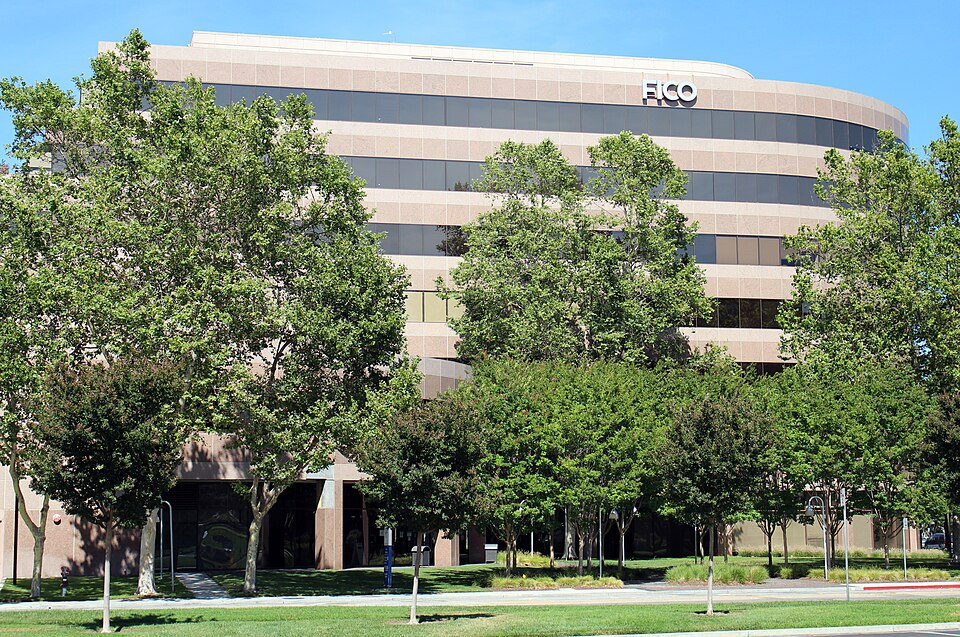
\includegraphics[height=0.40\textheight]{ch12_fico_hq_2020.jpg}\\[1mm]
\imgcap{Sediul FICO, San Jose, California}
\imgcredit{https://commons.wikimedia.org/wiki/File:Ficoheadquarters.jpg}{Foto: Coolcaesar (2020); CC BY-SA 4.0; Wikimedia Commons}
\end{column}
\end{columns}
\end{frame}

\begin{frame}{PD, LGD, EAD și pierderea așteptată}
\itemsize{\small}
\begin{itemize}
    \item Trei parametri de risc ai unui credit (Basel II, \refBCBS)
    \begin{itemize}
        \item \textbf{PD}: probabilitatea de nerambursare într-un an
        \item \textbf{LGD} (loss given default): partea din expunere pierdută în caz de nerambursare, după recuperări
        \item \textbf{EAD} (exposure at default): suma datorată în momentul nerambursării
    \end{itemize}
    \item \textbf{Pierderea așteptată}: $\mathrm{EL} = \mathrm{PD} \times \mathrm{LGD} \times \mathrm{EAD}$ (cu PD și LGD independente)
    \begin{itemize}
        \item \textbf{Exemplu}: un credit de 100\,000 de lei cu PD $= 2\%$, LGD $= 45\%$: EL $= 0{,}02 \times 0{,}45 \times 100\,000 = 900$ lei
        \item EL este un cost al activității: intră în dobîndă și este acoperită prin provizioane
    \end{itemize}
    \item Capitalul acoperă \textbf{pierderea neașteptată}: pierderile de peste EL într-un an prost
\end{itemize}
\end{frame}

\begin{frame}{Formula de capital IRB din Basel}
\itemsize{\footnotesize}
\begin{columns}[T]
\begin{column}{0.62\textwidth}
\begin{itemize}
    \item Abordarea \textbf{IRB} (internal ratings-based): banca estimează PD (și eventual LGD, EAD); autoritatea de reglementare dă formula \refBCBS, ¶328--330
    \begin{itemize}
        \item $K = \mathrm{LGD}\left[\Phi\!\left(\dfrac{\Phi^{-1}(\mathrm{PD}) + \sqrt{R}\,\Phi^{-1}(0{,}999)}{\sqrt{1 - R}}\right) - \mathrm{PD}\right]$; RWA $= 12{,}5\,K\,$EAD
        \item $K$: capitalul pe unitatea de EAD; $\Phi$, $\Phi^{-1}$: funcția de repartiție $N(0,1)$ și inversa ei; 0,999: un an prost apare o dată la 1000 de ani
        \item $R$: corelația debitorilor cu un factor comun; RWA (risk-weighted assets): activele ponderate la risc, din care banca deține cel puțin 8\%
    \end{itemize}
    \item Logica \refGordy: termenul din $\Phi(\cdot)$ este PD într-un an al cărui factor comun este depășit doar cu probabilitatea 0,1\%
    \begin{itemize}
        \item deci $K$ este VaR 0,1\% al pierderii din credit minus EL: pierderea neașteptată (\sfmchlink{https://danpele.github.io/SFM/RO/Cursuri/capitol10_var_es_backtesting.pdf}{Capitolul 10})
    \end{itemize}
\end{itemize}
\end{column}
\begin{column}{0.34\textwidth}
\centering
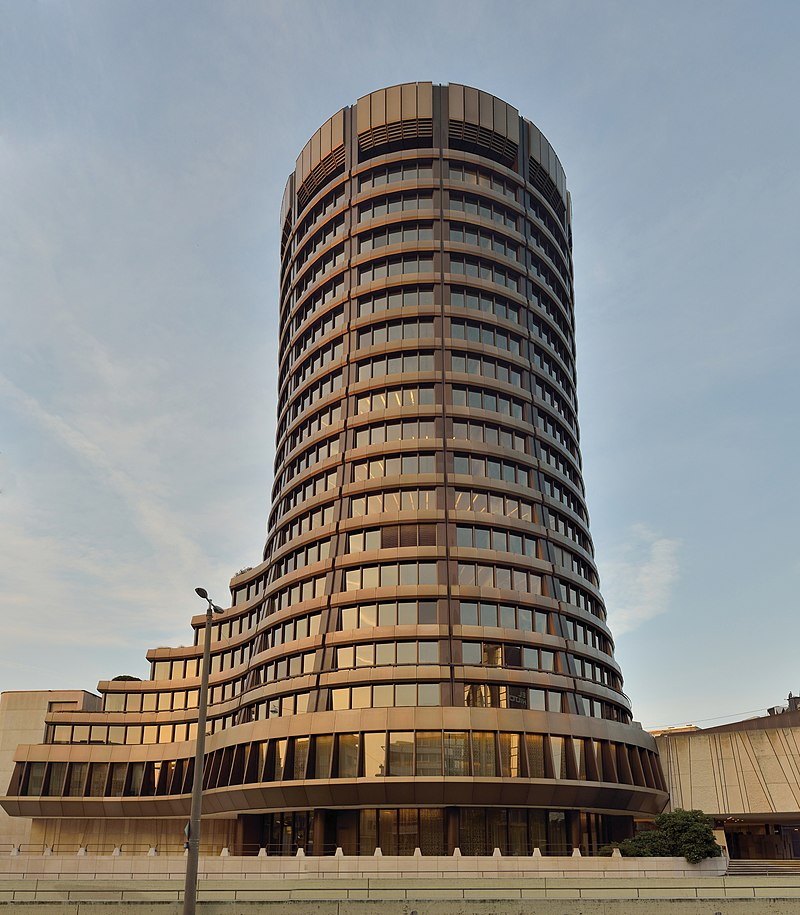
\includegraphics[height=0.40\textheight]{ch10_bis_tower_2014.jpg}\\[1mm]
\imgcap{Turnul BIS din Basel}
\imgcredit{https://commons.wikimedia.org/wiki/File:Basel_Committee_on_Banking_Supervision_-_BCBS.jpg}{Foto: Taxiarchos228 (2014); CC BY-SA 4.0; Wikimedia Commons}
\end{column}
\end{columns}
\end{frame}

\begin{frame}{PD în ani buni și în ani proști: modelul cu un factor}
\itemsize{\footnotesize}
\begin{center}
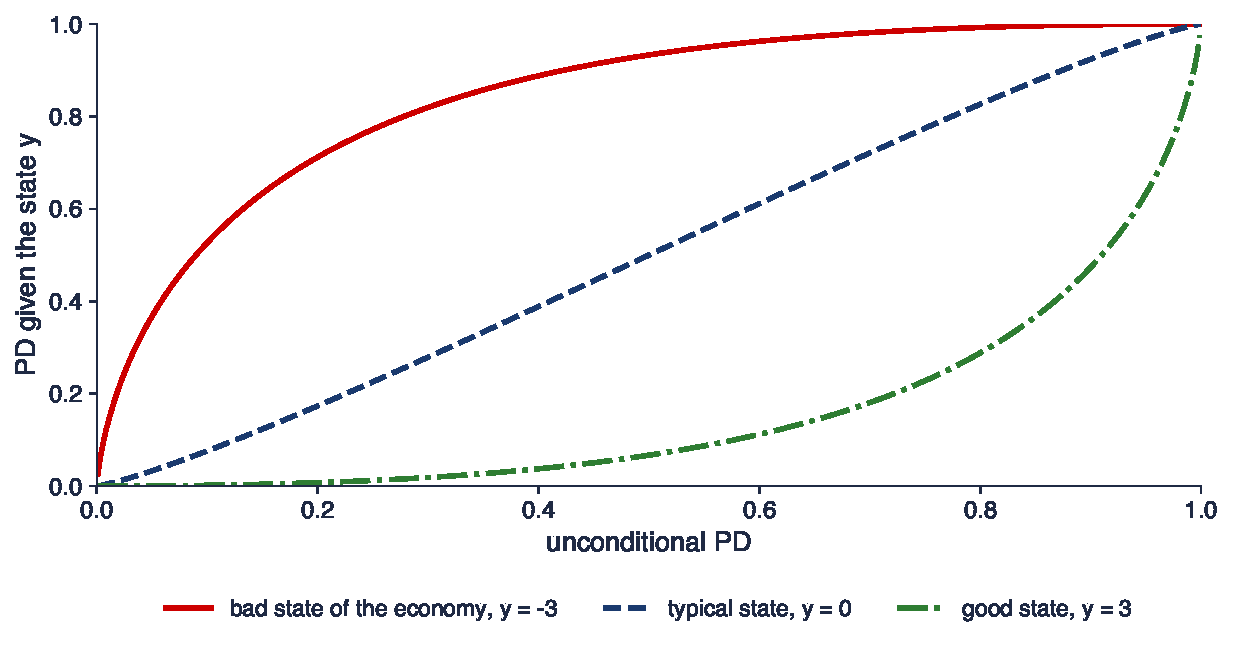
\includegraphics[width=0.97\textwidth,height=0.46\textheight,keepaspectratio]{sfm_ch12_conditional_pd.pdf}
\end{center}
\vspace{-0.25cm}
\begin{itemize}
    \item Debitorul $i$ intră în nerambursare dacă $\sqrt{\rho}\,Y + \sqrt{1 - \rho}\,\varepsilon_i < \Phi^{-1}(\mathrm{PD})$; $Y$: starea economiei; dat fiind $Y = y$: PD$(y) = \Phi\big((\Phi^{-1}(\mathrm{PD}) - \sqrt{\rho}\,y)/\sqrt{1 - \rho}\big)$, $\rho = 0{,}2$
    \item $\varepsilon_i$: șocul propriu al debitorului; $Y$ și $\varepsilon_i$ independente, $N(0,1)$; $\rho$: ponderea factorului comun
    \item Interpretare: un credit cu PD $= 2\%$ intră în nerambursare cu probabilitatea 21{,}3\% într-un an prost ($y = -3$), 1{,}1\% într-un an obișnuit și aproape niciodată într-un an bun; IRB folosește $y = \Phi^{-1}(0{,}001)$
\end{itemize}
\sfmquantlet{Ch_12}{SFM_ch12_validation_irb}
\end{frame}

\begin{frame}{Exemplu rezolvat: capitalul IRB al unui credit de retail}
\itemsize{\footnotesize}
\begin{itemize}
    \item Alte expuneri de retail: $R = 0{,}03\,w + 0{,}16\,(1 - w)$, $w = (1 - e^{-35\,\mathrm{PD}})/(1 - e^{-35})$ \refBCBS, ¶330
    \begin{itemize}
        \item $w \in [0, 1]$ crește cu PD, deci $R$ scade de la 0,16 (credite foarte sigure) la 0,03 (credite foarte riscante)
        \item PD $= 2\%$: $R = 0{,}095$; $\Phi^{-1}(0{,}02) = -2{,}054$, $\Phi^{-1}(0{,}999) = 3{,}090$
    \end{itemize}
    \item \textbf{Pas cu pas}
    \begin{itemize}
        \item argumentul: $(-2{,}054 + \sqrt{0{,}095} \times 3{,}090)/\sqrt{1 - 0{,}095} = -1{,}160$; $\Phi(-1{,}160) = 12{,}31\%$: PD într-un an prost
        \item $K = 0{,}45 \times (12{,}31\% - 2\%) = 4{,}64\%$ din EAD: 4\,639 lei pentru un credit de 100\,000 de lei
        \item RWA $= 12{,}5 \times 4\,639 = 57\,986$ lei: o pondere de risc de 58\%
    \end{itemize}
    \item Interpretare: EL ($900$ lei) intră în preț; capitalul ($4\,639$ lei) absoarbe un an în care nerambursările ajung la 12{,}31\% în loc de 2\%
\end{itemize}
\end{frame}

\begin{frame}{Pierderea așteptată și capitalul IRB în funcție de PD}
\itemsize{\footnotesize}
\begin{center}
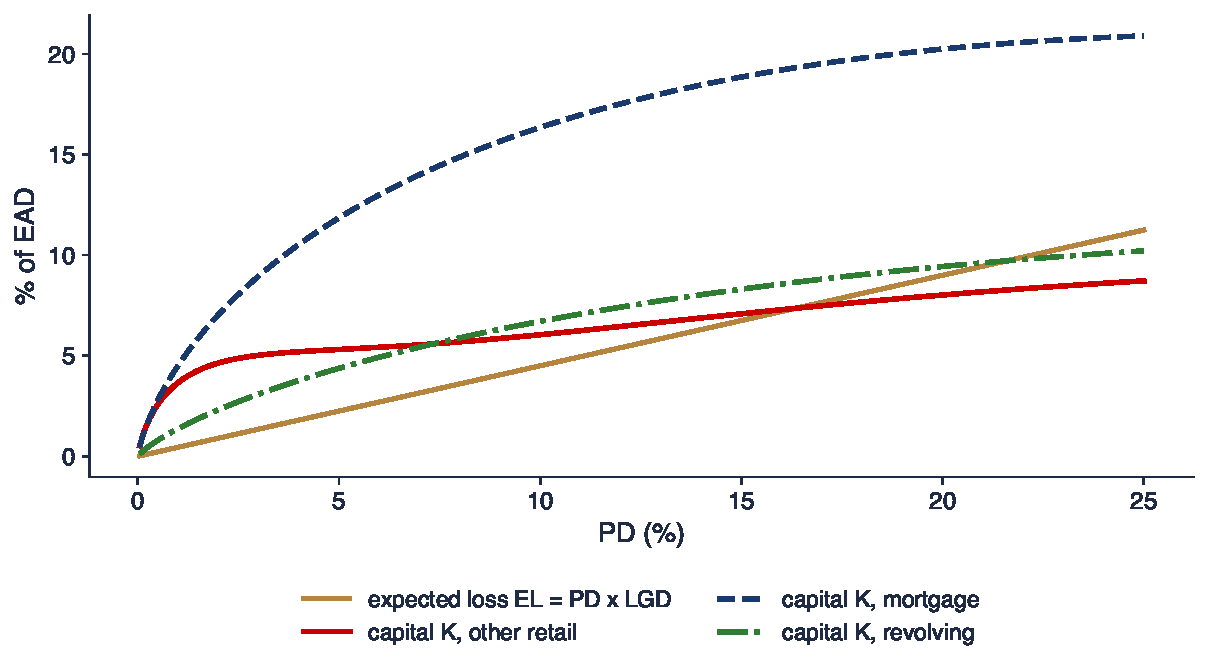
\includegraphics[width=0.97\textwidth,height=0.50\textheight,keepaspectratio]{sfm_ch12_irb.pdf}
\end{center}
\vspace{-0.25cm}
\begin{itemize}
    \item LGD $= 45\%$; capitalul $K$ pentru alte expuneri de retail ($R$ de la 0,16 la 0,03), credite ipotecare ($R = 0{,}15$) și expuneri revolving ($R = 0{,}04$)
    \item Interpretare: EL crește liniar cu PD; $K$ crește repede la PD mici și apoi se aplatizează, deoarece un credit foarte riscant este în mare parte o pierdere așteptată (inclusă în preț)
\end{itemize}
\sfmquantlet{Ch_12}{SFM_ch12_validation_irb}
\end{frame}

\begin{frame}{Recapitulare: scorul de credit: definiție}
\itemsize{\small}
\begin{itemize}
    \item Un scor ordonează solicitanții după risc; o PD dă și nivelul riscului
    \item EL $=$ PD $\times$ LGD $\times$ EAD intră în preț; capitalul Basel acoperă pierderea neașteptată (VaR 0,1\% al creditului minus EL)
    \item Scoringul statistic a început cu analiza discriminantă a lui Fisher (Durand, 1941)
\end{itemize}
\end{frame}


%=============================================================================
\section{Datele de nerambursare}
%=============================================================================

\begin{frame}{Datele South German Credit}
\itemsize{\small}
\begin{itemize}
    \item 1\,000 de credite de consum ale unei mari bănci regionale din sudul Germaniei, 1973--1975 \refSGC; \refGroemping
    \begin{itemize}
        \item rezultatul: contractul a fost respectat (bun-platnic) sau nu (rău-platnic, \textbf{nerambursare} $= 1$): 300 de credite neperformante și 700 performante
        \item 20 de variabile: contul curent, durata, istoricul de credit, destinația, suma (DM, mărci germane), economiile, vechimea în muncă, vîrsta și altele
    \end{itemize}
    \item Un \textbf{eșantion stratificat}: creditele neperformante sînt puternic suprareprezentate; rata lor în bancă era de aproximativ 5\% \refGroemping
    \begin{itemize}
        \item toți debitorii trecuseră de verificările băncii: solicitanții respinși lipsesc (reject inference, secțiunea 8)
        \item costul acceptării unui credit neperformant este stabilit la de cinci ori costul respingerii unuia performant
    \end{itemize}
    \item Licența CC BY 4.0; salvate o singură dată în repository-ul cursului (data/credit)
\end{itemize}
\end{frame}

\begin{frame}{O lecție despre verificarea datelor}
\itemsize{\small}
\begin{itemize}
    \item Datele au fost folosite zeci de ani în versiunea UCI „Statlog (German Credit)”, cu etichete greșite ale codurilor \refGroemping
    \begin{itemize}
        \item în acea versiune, „fără cont curent” era grupul cel mai sigur: 394 de credite, 11{,}7\% neperformante
        \item în datele corectate, acele 394 de credite au un sold de cel puțin 200 DM sau un cont de salariu; „fără cont curent” este grupul cel mai riscant (49{,}3\% neperformante)
    \end{itemize}
    \item Cifrele erau corecte, etichetele greșite: fiecare model funcționa, fiecare interpretare a acestei variabile era inversată
    \begin{itemize}
        \item verificări: comparăm tabelele de frecvențe cu sursa originală (aici cartea lui Fahrmeir și Hamerle) și ne întrebăm dacă semnele au sens economic
    \end{itemize}
    \item Folosim în tot capitolul datele corectate South German Credit
\end{itemize}
\end{frame}

\begin{frame}{Rata creditelor neperformante după contul curent}
\itemsize{\footnotesize}
\begin{center}
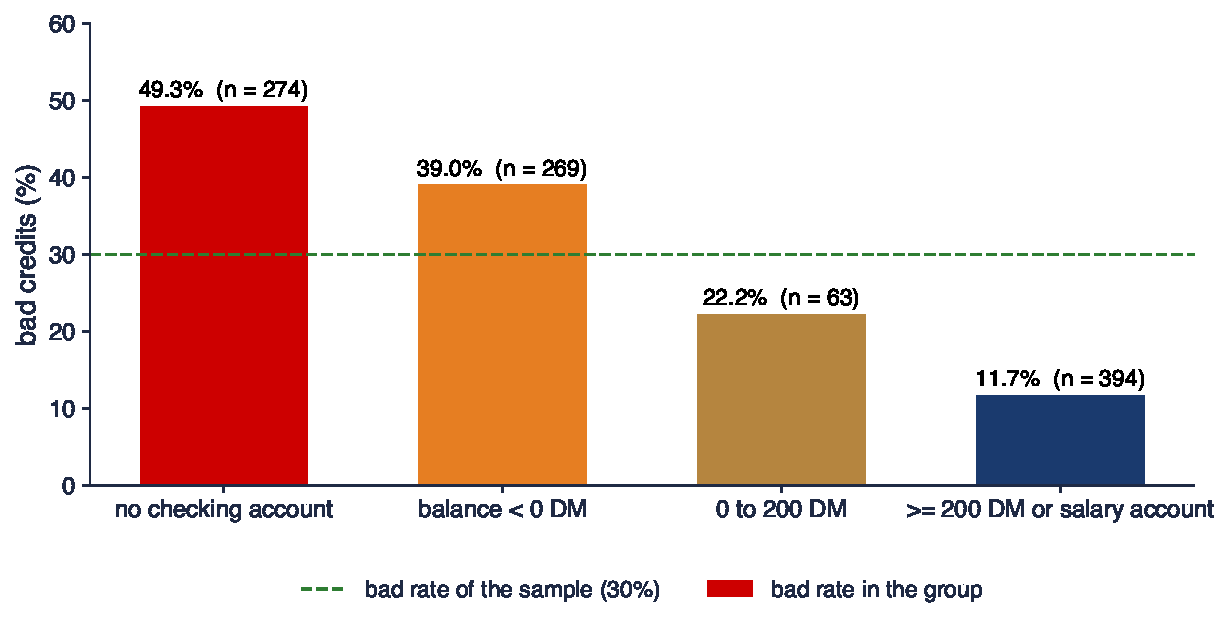
\includegraphics[width=0.97\textwidth,height=0.50\textheight,keepaspectratio]{sfm_ch12_default_by_status.pdf}
\end{center}
\vspace{-0.25cm}
\begin{itemize}
    \item Ponderea creditelor neperformante în fiecare grup; linia întreruptă: media eșantionului, 30\%
    \item Interpretare: riscul scade de la 49{,}3\% (fără cont) la 11{,}7\% (sold de cel puțin 200 DM): o singură variabilă separă deja bine solicitanții
\end{itemize}
\sfmquantlet{Ch_12}{SFM_ch12_woe_iv}
\end{frame}

\begin{frame}{Dezechilibrul claselor și suprareprezentarea}
\itemsize{\small}
\begin{itemize}
    \item Nerambursările sînt rare: cîteva procente din creditele unei bănci; un eșantion cu puțini rău-platnici spune puțin despre ei
    \begin{itemize}
        \item de aceea băncile suprareprezintă rău-platnicii (aici 30\% în loc de circa 5\%)
    \end{itemize}
    \item \textbf{Paradoxul acurateței}: regula „toți sînt bun-platnici” are dreptate pentru 70\% din acest eșantion și pentru 77{,}9\% din datele din Taiwan
    \begin{itemize}
        \item deci acuratețea singură este o măsură slabă; avem nevoie de măsuri care privesc separat rău-platnicii și bun-platnicii (secțiunea 7)
    \end{itemize}
    \item \textbf{Datele cardurilor de credit din Taiwan} \refTW; \refYL: 30\,000 de deținători de card, nerambursarea plății din octombrie 2005, 22{,}1\% nerambursări
    \begin{itemize}
        \item variabile: limita de credit, vîrsta, starea plăților din aprilie--septembrie 2005, facturile și plățile; le folosim pentru calibrare și echitate
    \end{itemize}
\end{itemize}
\end{frame}

\begin{frame}{Eșantionul de estimare și eșantionul de test}
\itemsize{\small}
\begin{itemize}
    \item \textbf{Împărțire stratificată}: 700 de credite pentru estimare, 300 pentru test, cu 30\% rău-platnici în ambele
    \begin{itemize}
        \item orice alegere (intervale, WoE, variabile, coeficienți) se face doar pe eșantionul de estimare
        \item eșantionul de test se folosește o singură dată, la final: joacă rolul viitorilor solicitanți
    \end{itemize}
    \item \textbf{Leakage} (scurgerea de informație): informație din eșantionul de test care intră în model, de exemplu intervale alese pe toate datele
    \begin{itemize}
        \item face rezultatul testului prea optimist; cu 300 de credite de test, o singură împărțire este și zgomotoasă, așa că adăugăm validarea încrucișată (secțiunea 7)
    \end{itemize}
\end{itemize}
\end{frame}

\begin{frame}{Recapitulare: datele de nerambursare}
\itemsize{\small}
\begin{itemize}
    \item South German Credit: 1\,000 de credite, 30\% neperformante prin construcție; versiunea larg folosită avea etichete greșite
    \item Dezechilibrul face acuratețea înșelătoare; suprareprezentarea schimbă nivelul PD, nu ordonarea
    \item Estimăm pe eșantionul de estimare, judecăm pe eșantionul de test
\end{itemize}
\end{frame}


%=============================================================================
\section{Weight of Evidence și Information Value}
%=============================================================================

\begin{frame}{Weight of Evidence (WoE)}
\itemsize{\footnotesize}
\begin{itemize}
    \item Împărțim o variabilă în intervale (clase) $i = 1, \dots, m$; $g_i$, $b_i$: bun-platnicii și rău-platnicii din intervalul $i$; $G$, $B$: totalurile lor
    \begin{itemize}
        \item $\mathrm{WoE}_i = \ln\dfrac{g_i/G}{b_i/B}$: logaritmul raportului dintre ponderea bun-platnicilor și ponderea rău-platnicilor în interval
    \end{itemize}
    \item Sensul: $\mathrm{WoE}_i = \ln\dfrac{g_i}{b_i} - \ln\dfrac{G}{B}$: logaritmul șansei de a fi bun-platnic în interval minus cel din întregul eșantion
    \begin{itemize}
        \item $\mathrm{WoE} > 0$: mai sigur decît media; $\mathrm{WoE} < 0$: mai riscant; $\mathrm{WoE} = 0$: nicio informație
        \item un interval fără bun-platnici sau fără rău-platnici ar da $\pm\infty$: adăugăm 0,5 la ambele frecvențe
    \end{itemize}
    \item \textbf{Information Value}: $\mathrm{IV} = \sum_i \left(\dfrac{g_i}{G} - \dfrac{b_i}{B}\right)\mathrm{WoE}_i \ge 0$
    \begin{itemize}
        \item o divergență Kullback--Leibler simetrică între distribuțiile bun-platnicilor și ale rău-platnicilor pe intervale
        \item regula practică \refSiddiqi: sub 0,02 inutilă, 0,02--0,1 slabă, 0,1--0,3 medie, peste 0,3 puternică
    \end{itemize}
\end{itemize}
\end{frame}

\begin{frame}{Exemplu rezolvat: WoE și IV pentru contul curent}
\itemsize{\footnotesize}
\begin{center}
\scriptsize
\begin{tabular}{lrrrrrr}
\toprule
Contul curent & bun-pl. & rău-pl. & $g_i/G$ & $b_i/B$ & WoE & termen IV \\
\midrule
fără cont curent & 139 & 135 & $0{,}199$ & $0{,}450$ & $-0{,}818$ & $0{,}206$ \\
sold $<$ 0 DM & 164 & 105 & $0{,}234$ & $0{,}350$ & $-0{,}401$ & $0{,}046$ \\
0--200 DM & 49 & 14 & $0{,}070$ & $0{,}047$ & $0{,}405$ & $0{,}009$ \\
$\ge$ 200 DM sau salariu & 348 & 46 & $0{,}497$ & $0{,}153$ & $1{,}176$ & $0{,}404$ \\
total & 700 & 300 & 1 & 1 & & $0{,}666$ \\
\bottomrule
\end{tabular}
\end{center}
\begin{itemize}
    \item \textbf{Pas cu pas}, ultimul rînd: $g/G = 348/700 = 0{,}497$, $b/B = 46/300 = 0{,}153$
    \begin{itemize}
        \item WoE $= \ln(0{,}497/0{,}153) = 1{,}176$; termenul IV $= (0{,}497 - 0{,}153) \times 1{,}176 = 0{,}404$
    \end{itemize}
    \item Interpretare: IV $= 0{,}666 > 0{,}3$: o variabilă puternică; WoE scade monoton de la grupul cel mai sigur la cel mai riscant
\end{itemize}
\end{frame}

\begin{frame}{Discretizarea (binning): reguli practice}
\itemsize{\small}
\begin{itemize}
    \item Rolul intervalelor: surprind efectele neliniare, limitează influența valorilor extreme și dau fiecărui solicitant un tabel mic de puncte
    \begin{itemize}
        \item variabile numerice: cîteva intervale (aici durata $\le 12$, 13--18, 19--24, 25--36, $> 36$ de luni); categoriale: categoriile
    \end{itemize}
    \item Reguli \refSiddiqi; \refTCE
    \begin{itemize}
        \item cel puțin aproximativ 5\% din eșantion în fiecare interval; unim categoriile mici
        \item WoE trebuie să varieze într-un mod cu sens economic (adesea monoton)
        \item intervalele și WoE se estimează pe eșantionul de estimare și se aplică neschimbate noilor solicitanți
    \end{itemize}
    \item O variabilă WoE intră în modelul logit cu un singur coeficient: scorecard-ul rămîne aditiv și ușor de citit
\end{itemize}
\end{frame}

\begin{frame}{WoE pentru durata creditului}
\itemsize{\footnotesize}
\begin{center}
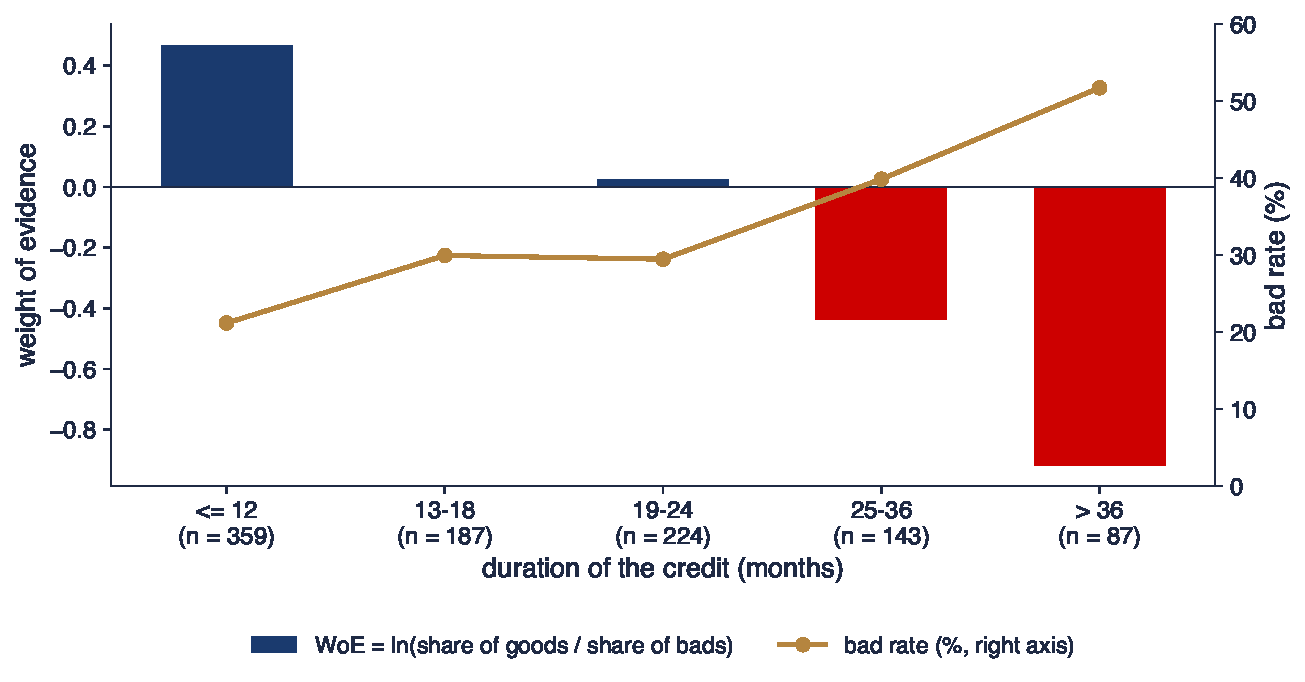
\includegraphics[width=0.97\textwidth,height=0.50\textheight,keepaspectratio]{sfm_ch12_woe_duration.pdf}
\end{center}
\vspace{-0.25cm}
\begin{itemize}
    \item Eșantionul complet; bare: WoE pentru fiecare interval de durată; linia: rata creditelor neperformante (axa din dreapta); IV $= 0{,}182$ (medie)
    \item Interpretare: creditele de pînă la un an sînt mai sigure (WoE $= 0{,}47$, 21\% neperformante); peste trei ani, rata ajunge la 52\% (WoE $= -0{,}92$); 13--24 de luni sînt în medie
\end{itemize}
\sfmquantlet{Ch_12}{SFM_ch12_woe_iv}
\end{frame}

\begin{frame}{Information Value pentru cele 20 de variabile}
\itemsize{\footnotesize}
\begin{center}
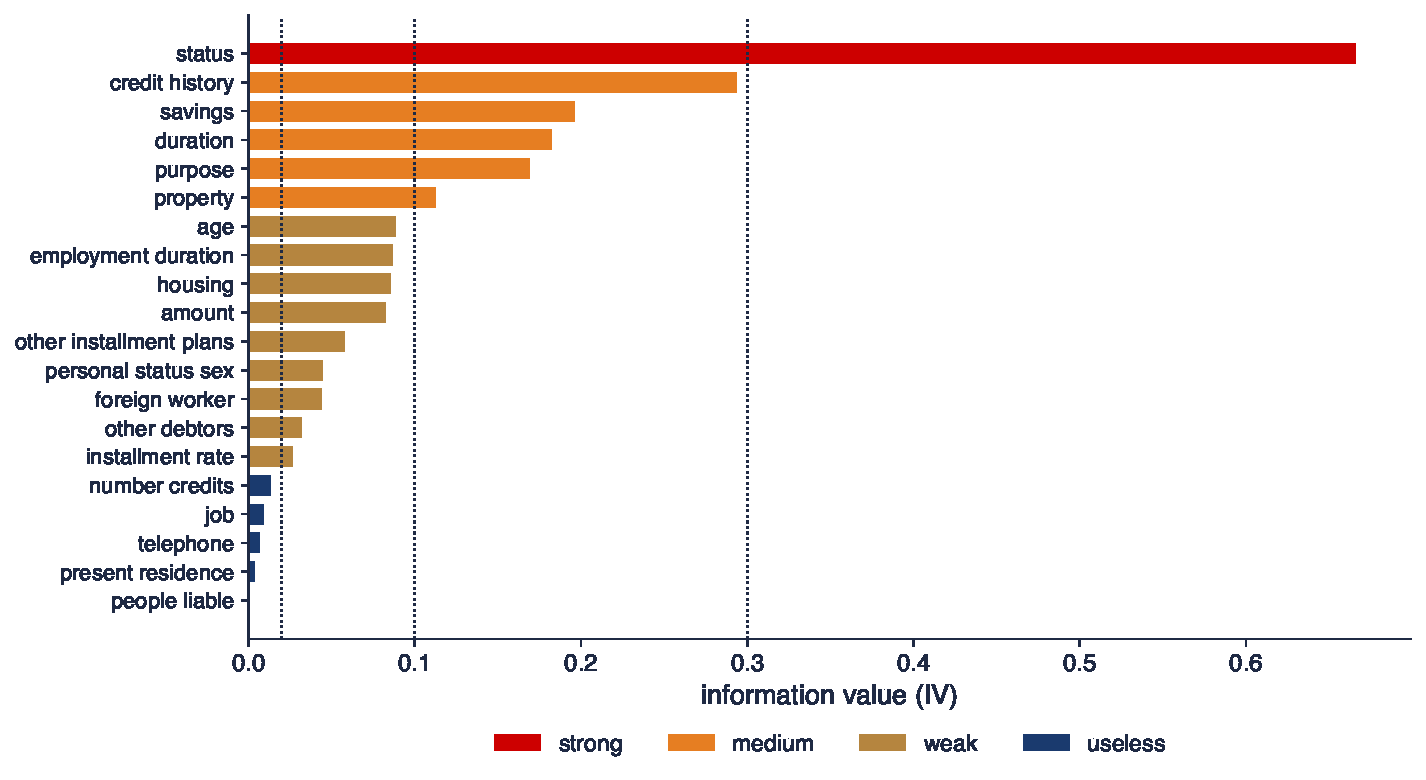
\includegraphics[width=0.97\textwidth,height=0.48\textheight,keepaspectratio]{sfm_ch12_iv.pdf}
\end{center}
\vspace{-0.25cm}
\begin{itemize}
    \item Eșantionul complet; linii punctate: pragurile 0,02; 0,1 și 0,3; pe eșantionul de estimare, 6 variabile au IV $\ge 0{,}1$ și intră în scorecard
    \item Interpretare: contul curent (IV $= 0{,}666$) și istoricul de credit ($0{,}293$) domină; telefonul, vechimea la adresă și persoanele în întreținere nu aduc informație
    \item IV privește o singură variabilă: două variabile puternice, dar corelate, nu își adună informația
\end{itemize}
\sfmquantlet{Ch_12}{SFM_ch12_woe_iv}
\end{frame}

\begin{frame}{Recapitulare: Weight of Evidence și Information Value}
\itemsize{\small}
\begin{itemize}
    \item WoE: logaritmul raportului dintre ponderea bun-platnicilor și a rău-platnicilor într-un interval; pozitiv înseamnă mai sigur decît media
    \item IV ordonează variabilele; 0,1 și 0,3 marchează variabilele medii și puternice
    \item Intervalele, WoE și selecția variabilelor aparțin eșantionului de estimare
\end{itemize}
\end{frame}


%=============================================================================
\section{Regresia logistică}
%=============================================================================

\begin{frame}{Șansa (odds) și logaritmul șansei}
\itemsize{\small}
\begin{itemize}
    \item Un model liniar $P(Y = 1) = \beta_0 + x^\top\beta$ poate da probabilități sub 0 sau peste 1
    \begin{itemize}
        \item modelăm o transformare a lui $p$ care poate lua orice valoare reală
    \end{itemize}
    \item \textbf{Șansa} (odds) de nerambursare: $\dfrac{p}{1 - p} \in (0, \infty)$; \textbf{logaritmul șansei} (logit): $\ln\dfrac{p}{1 - p} \in (-\infty, \infty)$
    \begin{itemize}
        \item $p = 0{,}20$: șansa $= 0{,}2/0{,}8 = 0{,}25$ (o nerambursare la patru credite rambursate); logaritmul șansei $= \ln 0{,}25 = -1{,}386$
        \item $p = 0{,}5$: șansa 1, logaritmul șansei 0; logit-ul este simetric: $\mathrm{logit}(1 - p) = -\mathrm{logit}(p)$
    \end{itemize}
    \item Bancherii vorbesc adesea despre \textbf{șansa bun:rău} $(1 - p)/p$: aici 4:1
\end{itemize}
\end{frame}

\begin{frame}{Modelul logit}
\itemsize{\small}
\begin{itemize}
    \item $\ln\dfrac{p_i}{1 - p_i} = \beta_0 + x_i^\top\beta = \eta_i$, \quad $p_i = P(Y_i = 1 \mid x_i) = \dfrac{1}{1 + e^{-\eta_i}}$ \refCox
    \begin{itemize}
        \item $\beta_0$: termenul liber; $\eta_i$: predictorul liniar, logaritmul șansei solicitantului $i$
    \end{itemize}
    \item \textbf{Verosimilitatea maximă} (\sfmchlink{https://danpele.github.io/SFM/RO/Cursuri/capitol6_selectia_modelului_managementul_riscului.pdf}{Capitolul 6}): $\ell(\beta) = \sum_i [y_i\ln p_i + (1 - y_i)\ln(1 - p_i)]$
    \begin{itemize}
        \item condiția de ordinul întîi $\sum_i (y_i - p_i)x_i = 0$: fără formulă explicită, se rezolvă prin Newton--Raphson
        \item erorile standard din inversa lui $\sum_i p_i(1 - p_i)x_ix_i^\top$; testul Wald $z = \hat\beta_j/\mathrm{se}(\hat\beta_j)$
    \end{itemize}
    \item Modelul logit este folosit și pentru falimentul companiilor, începînd cu \refOhlson; modelul probit folosește $\Phi(\eta)$ în locul funcției logistice
    \begin{itemize}
        \item logit și probit dau aproape aceleași PD; logit-ul are interpretarea prin șanse
    \end{itemize}
\end{itemize}
\end{frame}

\begin{frame}{O curbă logistică: PD și durata}
\itemsize{\footnotesize}
\begin{center}
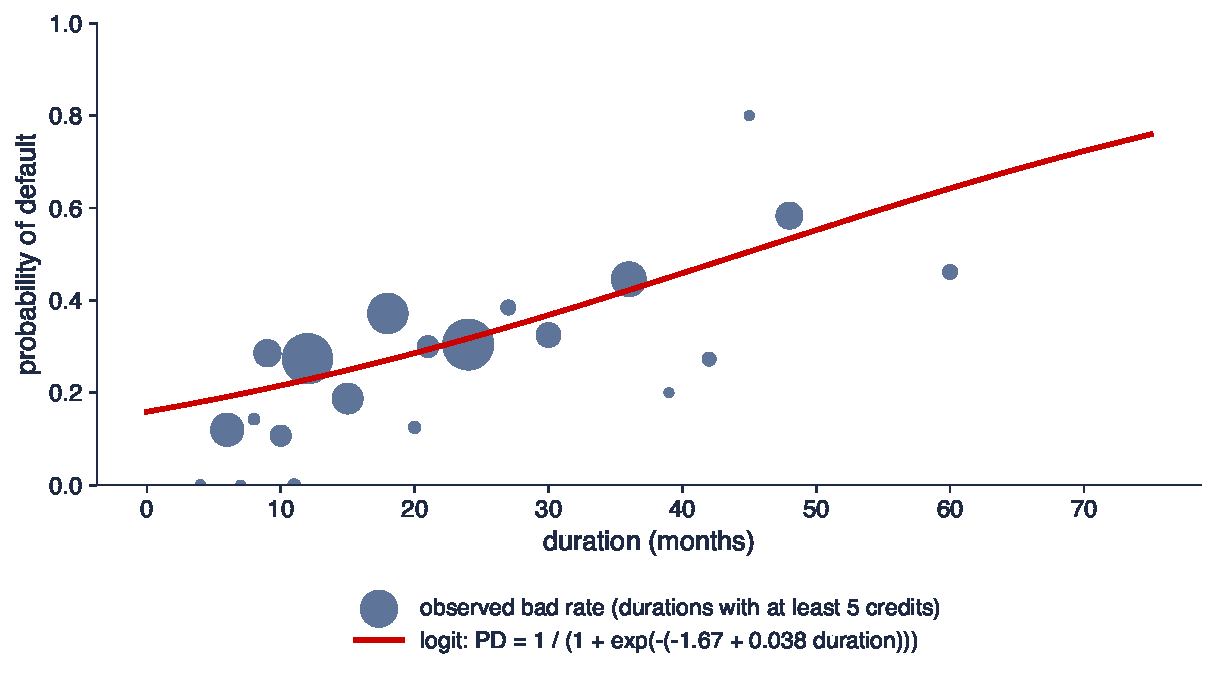
\includegraphics[width=0.97\textwidth,height=0.50\textheight,keepaspectratio]{sfm_ch12_logistic_curve.pdf}
\end{center}
\vspace{-0.25cm}
\begin{itemize}
    \item Logit doar cu durata: $\hat\beta_0 = -1{,}666$, $\hat\beta_1 = 0{,}0375$ pe lună (se $0{,}0057$); punctele: ratele observate
    \item Interpretare: fiecare an în plus înmulțește șansa de nerambursare cu $e^{12 \times 0{,}0375} = 1{,}57$; PD crește de la 22{,}9\% la 12 luni la 53{,}4\% la 48 de luni
\end{itemize}
\sfmquantlet{Ch_12}{SFM_ch12_logit_lda}
\end{frame}

\begin{frame}{Interpretarea coeficienților}
\itemsize{\small}
\begin{itemize}
    \item $\beta_j$: modificarea \textbf{logaritmului șansei} cînd $x_j$ crește cu o unitate, celelalte variabile fiind fixe
    \begin{itemize}
        \item $e^{\beta_j}$: \textbf{raportul șanselor} (odds ratio): șansa se înmulțește cu $e^{\beta_j}$; $100(e^{\beta_j} - 1)\%$ este modificarea șansei
        \item un interval de încredere de 95\%: $\exp(\hat\beta_j \pm 1{,}96\,\mathrm{se})$
    \end{itemize}
    \item Efectul asupra \textbf{probabilității} depinde de poziția solicitantului
    \begin{itemize}
        \item $\partial p/\partial x_j = p(1 - p)\beta_j$: maxim la $p = 0{,}5$, mic pentru solicitanții foarte siguri sau foarte riscanți
    \end{itemize}
    \item O variabilă indicator (0/1): $e^{\beta_j}$ compară șansa grupului cu cea a grupului de referință
    \begin{itemize}
        \item interpretarea cere un model care conține variabilele relevante: o variabilă omisă schimbă coeficienții
    \end{itemize}
\end{itemize}
\end{frame}

\begin{frame}{Un model logit mic pe eșantionul complet}
\itemsize{\footnotesize}
\begin{center}
\scriptsize
\begin{tabular}{lrrrrc}
\toprule
Variabila & $\hat\beta$ & se & $z$ & p & raportul șanselor (CI 95\%) \\
\midrule
termenul liber & $-2{,}101$ & $0{,}311$ & $-6{,}75$ & $<$\,0{,}001 &  \\
durata (ani) & $0{,}385$ & $0{,}092$ & $4{,}17$ & $<$\,0{,}001 & $1{,}47$ ($1{,}23$--$1{,}76$) \\
vîrsta (decenii) & $-0{,}159$ & $0{,}069$ & $-2{,}30$ & 0{,}022 & $0{,}85$ ($0{,}74$--$0{,}98$) \\
suma (1000 DM) & $0{,}029$ & $0{,}032$ & $0{,}90$ & 0{,}368 & $1{,}03$ ($0{,}97$--$1{,}10$) \\
fără cont curent & $1{,}859$ & $0{,}188$ & $9{,}89$ & $<$\,0{,}001 & $6{,}42$ ($4{,}44$--$9{,}28$) \\
sold $<$ 0 DM & $1{,}338$ & $0{,}192$ & $6{,}99$ & $<$\,0{,}001 & $3{,}81$ ($2{,}62$--$5{,}55$) \\
\bottomrule
\end{tabular}
\end{center}
\begin{itemize}
    \item $n = 1\,000$; log-verosimilitatea $-526{,}1$ față de $-610{,}9$ doar cu termenul liber: LR $= 169{,}6$ cu 5 grade de libertate
    \item Grupul de referință al indicatorilor de cont: un sold nenegativ (0--200 DM, sau cel puțin 200 DM ori cont de salariu)
\end{itemize}\sfmquantlet{Ch_12}{SFM_ch12_logit_lda}
\end{frame}

\begin{frame}{Rapoartele șanselor cu intervale de încredere}
\itemsize{\footnotesize}
\begin{columns}[T]
\begin{column}{0.54\textwidth}
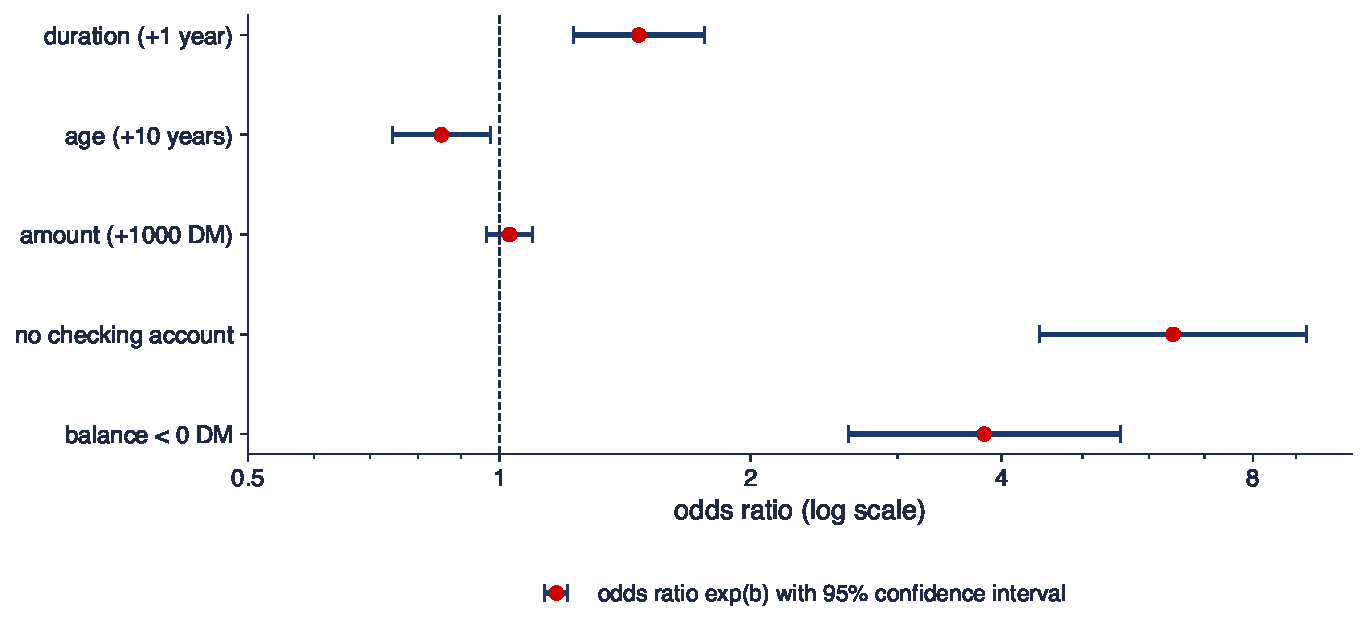
\includegraphics[width=\textwidth,height=0.55\textheight,keepaspectratio]{sfm_ch12_odds_ratios.pdf}
\end{column}
\begin{column}{0.44\textwidth}
\begin{itemize}
    \item Fiecare punct: $e^{\hat\beta}$; bare: intervale de 95\%; scală logaritmică; linia verticală: niciun efect (1)
    \item Interpretare: fără cont curent, șansa de nerambursare este de 6{,}42 ori cea a grupului de referință; un sold negativ o înmulțește cu 3{,}81
    \item Un an în plus de durată crește șansa cu 47\%; zece ani în plus de vîrstă o reduc cu aproximativ 15\%
    \item Suma nu este semnificativă odată ce durata este în model (cele două sînt corelate)
\end{itemize}
\end{column}
\end{columns}
\sfmquantlet{Ch_12}{SFM_ch12_logit_lda}
\end{frame}

\begin{frame}{Exemplu rezolvat: PD a unui solicitant}
\itemsize{\small}
\begin{itemize}
    \item Solicitantul: 36 de luni, 30 de ani, 4000 DM, fără cont curent; coeficienții din tabelul anterior, rotunjiți
    \begin{itemize}
        \item $\eta = -2{,}101 + 0{,}385 \times 3 + (-0{,}159) \times 3 + 0{,}029 \times 4 + 1{,}859$
        \item $\eta = -2{,}101 + 1{,}155 + (-0{,}477) + 0{,}116 + 1{,}859 = 0{,}552$
    \end{itemize}
    \item PD $= 1/(1 + e^{-0{,}552}) = 63{,}5\%$; șansa $e^{0{,}552} = 1{,}74$
    \begin{itemize}
        \item același solicitant cu un sold nenegativ: $\eta = -1{,}307$, PD $= 21{,}3\%$
        \item un an în plus de durată: $\Delta p \approx p(1 - p)\beta \approx 8{,}9$ puncte procentuale
    \end{itemize}
    \item Atenție: această PD se referă la un eșantion cu 30\% rău-platnici, nu la populația băncii (corecția pentru proporția a priori, peste două slide-uri)
\end{itemize}
\end{frame}

\begin{frame}{Scorecard-ul logit pe variabile WoE}
\itemsize{\footnotesize}
\begin{center}
\scriptsize
\begin{tabular}{lrrr}
\toprule
Variabila WoE & IV (estimare) & $\hat\beta$ & se \\
\midrule
termenul liber & & $-0{,}850$ & $0{,}095$ \\
contul curent & $0{,}591$ & $-0{,}829$ & $0{,}127$ \\
istoricul de credit & $0{,}215$ & $-0{,}675$ & $0{,}206$ \\
destinația creditului & $0{,}205$ & $-0{,}937$ & $0{,}217$ \\
economiile & $0{,}166$ & $-0{,}726$ & $0{,}246$ \\
durata & $0{,}159$ & $-1{,}082$ & $0{,}239$ \\
vechimea la angajator & $0{,}122$ & $-0{,}873$ & $0{,}265$ \\
\bottomrule
\end{tabular}
\end{center}
\begin{itemize}
    \item Eșantionul de estimare (700 de credite); fiecare variabilă este înlocuită cu WoE al intervalului ei; logit pentru nerambursare
    \begin{itemize}
        \item toți coeficienții sînt negativi: un WoE mai mare (interval mai sigur) reduce logaritmul șansei de nerambursare
        \item un coeficient de $-1$ ar însemna că variabila adaugă exact propriul WoE; valorile între $-0{,}7$ și $-1{,}1$ reflectă suprapunerea dintre variabile
    \end{itemize}
    \item Eșantionul de test: AUC $= 0{,}801$ (secțiunea 7); log-verosimilitatea în eșantion $-347{,}2$
\end{itemize}\sfmquantlet{Ch_12}{SFM_ch12_scorecard}
\end{frame}

\begin{frame}{Corecția pentru suprareprezentarea rău-platnicilor}
\itemsize{\small}
\begin{itemize}
    \item Dacă rău-platnicii și bun-platnicii sînt eșantionați cu rate diferite, se schimbă doar termenul liber al modelului logit
    \begin{itemize}
        \item $\ln\mathrm{șansa}_{\text{pop}} = \ln\mathrm{șansa}_{\text{eșantion}} + \ln\dfrac{\pi/(1 - \pi)}{\pi_s/(1 - \pi_s)}$; $\pi$: rata din populație, $\pi_s$: rata din eșantion
        \item pantele rămîn neschimbate: ordonarea solicitanților nu depinde de eșantionare
    \end{itemize}
    \item \textbf{Pas cu pas}: $\pi_s = 0{,}30$, $\pi = 0{,}05$: corecția $= \ln(0{,}05/0{,}95) - \ln(0{,}30/0{,}70) = -2{,}944 - (-0{,}847) = -2{,}097$
    \begin{itemize}
        \item o PD de 30\% în eșantion devine 5\%; o PD de 50\% devine 10{,}9\%
        \item solicitantul din exemplul lucrat: $0{,}552 - 2{,}097 = -1{,}545$, PD $= 17{,}6\%$ în populația băncii, în loc de 63{,}5\%
    \end{itemize}
    \item Interpretare: AUC și Gini nu sînt afectate de corecție; EL și capitalul sînt afectate
\end{itemize}
\end{frame}

\begin{frame}{Recapitulare: regresia logistică}
\itemsize{\small}
\begin{itemize}
    \item Modelul logit modelează liniar logaritmul șansei; $e^{\beta_j}$ este un raport al șanselor
    \item Se estimează prin verosimilitate maximă; efectul asupra PD este $p(1 - p)\beta_j$
    \item Suprareprezentarea mută doar termenul liber: o corectăm înainte de a folosi PD pentru EL sau capital
\end{itemize}
\end{frame}


%=============================================================================
\section{Analiza discriminantă liniară}
%=============================================================================

\begin{frame}{Ideea lui Fisher (1936)}
\itemsize{\footnotesize}
\begin{columns}[T]
\begin{column}{0.55\textwidth}
\begin{itemize}
    \item \refFisher: găsim combinația liniară $w^\top x$ care separă cel mai bine două grupuri
    \begin{itemize}
        \item a folosit măsurători ale florilor de iris; Durand a aplicat metoda creditelor cinci ani mai tîrziu
    \end{itemize}
    \item Criteriul Fisher: $J(w) = \dfrac{[w^\top(m_1 - m_0)]^2}{w^\top S_W w}$
    \begin{itemize}
        \item $m_0$, $m_1$: vectorii mediilor pentru bun-platnici și rău-platnici; $S_W$: matricea de covarianță comună din interiorul grupurilor
        \item maximul: $w \propto S_W^{-1}(m_1 - m_0)$ \refMVA, cap.~14
    \end{itemize}
    \item Criteriul nu cere nicio distribuție: este o proiecție care maximizează distanța dintre grupuri raportată la dispersia lor
\end{itemize}
\end{column}
\begin{column}{0.43\textwidth}
\begin{columns}[T]
\begin{column}{0.48\textwidth}
\centering

\includegraphics[height=0.34\textheight]{ch5_fisher_1913.jpg}\\[1mm]
\imgcap{R.A. Fisher, 1913}
\imgcredit{https://commons.wikimedia.org/wiki/File:Youngronaldfisher2.JPG}{Foto: autor necunoscut (1913); domeniu public; Wikimedia Commons}
\end{column}
\begin{column}{0.48\textwidth}
\centering

\includegraphics[height=0.30\textheight]{ch12_iris_versicolor.jpg}\\[1mm]
\imgcap{Iris versicolor}
\imgcredit{https://commons.wikimedia.org/wiki/File:Iris_versicolor_-20200620-RM-100933.jpg}{Foto: Ermell (2020); CC BY-SA 4.0; Wikimedia Commons}
\end{column}
\end{columns}
\end{column}
\end{columns}
\end{frame}

\begin{frame}{LDA ca model de probabilitate}
\itemsize{\footnotesize}
\begin{itemize}
    \item Presupunem $x \mid Y = k \sim N(m_k, \Sigma)$, aceeași $\Sigma$ în ambele grupuri, și probabilitatea a priori $\pi_1 = P(Y = 1)$
    \begin{itemize}
        \item Bayes: $\ln\dfrac{P(Y = 1 \mid x)}{P(Y = 0 \mid x)} = \underbrace{\ln\dfrac{\pi_1}{1 - \pi_1} - \tfrac12(m_1 + m_0)^\top w}_{c} + w^\top x$, \quad $w = \Sigma^{-1}(m_1 - m_0)$
        \item logaritmul șansei este \textbf{liniar în} $x$, exact ca în modelul logit; probabilitatea a priori intră doar în termenul liber
    \end{itemize}
    \item Diferența este în estimare
    \begin{itemize}
        \item LDA: folosim direct mediile de selecție și covarianța comună (formulă explicită)
        \item logit: maximizăm verosimilitatea condiționată a lui $Y$ dată fiind $x$; nicio ipoteză asupra distribuției lui $x$
    \end{itemize}
    \item Regula de clasificare: clasificăm solicitantul ca „rău-platnic” dacă $c + w^\top x > \ln(C_{FP}/C_{FN})$ (costuri, secțiunea 7)
\end{itemize}
\end{frame}

\begin{frame}{Exemplu rezolvat: direcția Fisher cu două variabile}
\itemsize{\footnotesize}
\begin{itemize}
    \item $x = $ (durata în luni, vîrsta în ani), eșantionul complet: 700 de bun-platnici, 300 de rău-platnici
    \begin{itemize}
        \item $m_0 = (19{,}21; 36{,}22)$, $m_1 = (24{,}86; 33{,}96)$, $m_1 - m_0 = (5{,}65; -2{,}26)$
        \item $S_W = \begin{pmatrix} 138{,}8 & -2{,}46 \\ -2{,}46 & 127{,}9 \end{pmatrix}$, $\det S_W = 17756$
    \end{itemize}
    \item \textbf{Pas cu pas}: $S_W^{-1} = \dfrac{1}{\det S_W}\begin{pmatrix} 127{,}9 & -(-2{,}46) \\ -(-2{,}46) & 138{,}8 \end{pmatrix}$, $w = S_W^{-1}(m_1 - m_0) = (0{,}0404; -0{,}0169)$
    \begin{itemize}
        \item logit cu aceleași două variabile: pantele $(0{,}0375; -0{,}0183)$
        \item raportul durată/vîrstă: LDA $-2{,}39$, logit $-2{,}05$: o lună de durată cîntărește cît aproximativ doi ani de vîrstă, în sens invers
    \end{itemize}
\end{itemize}
\end{frame}

\begin{frame}{Frontiera Fisher și frontiera logit}
\itemsize{\footnotesize}
\begin{center}
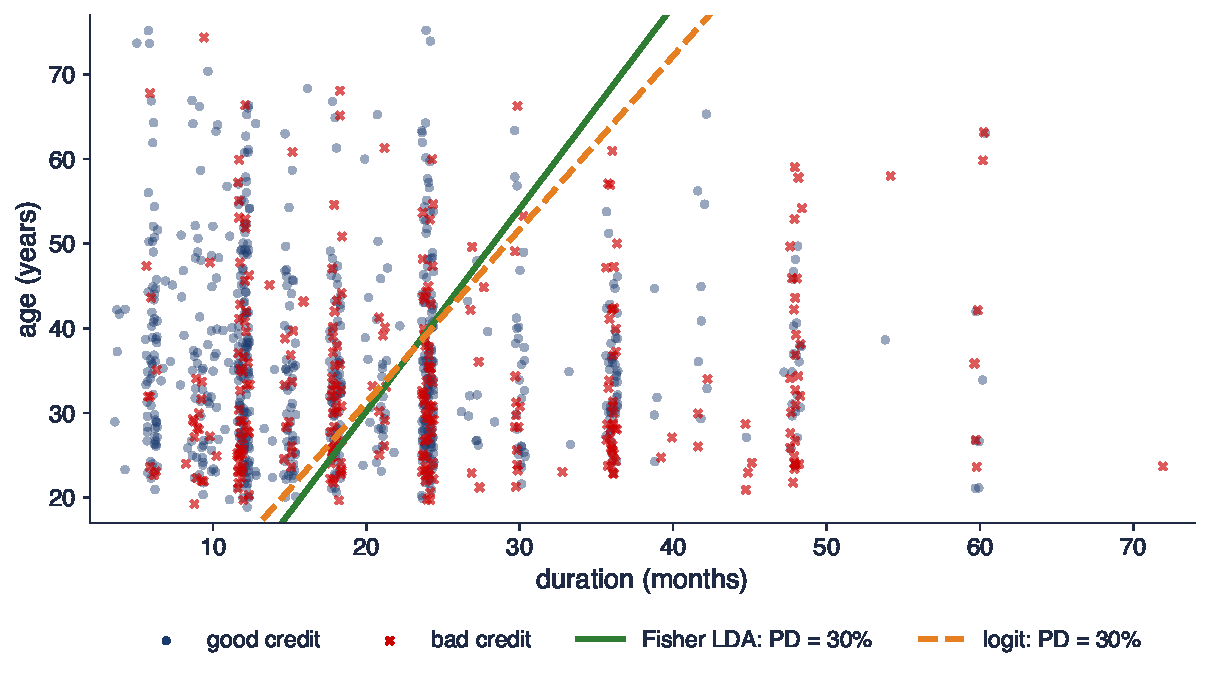
\includegraphics[width=0.97\textwidth,height=0.50\textheight,keepaspectratio]{sfm_ch12_lda_2d.pdf}
\end{center}
\vspace{-0.25cm}
\begin{itemize}
    \item Durata și vîrsta fiecărui credit (cu o mică perturbare); liniile: punctele cu PD $= 30\%$ (rata din eșantion) pentru LDA și pentru logit
    \item Interpretare: ambele frontiere sînt drepte cu aproape aceeași pantă; cei doi nori se suprapun mult, deci două variabile sînt departe de a fi suficiente
\end{itemize}
\sfmquantlet{Ch_12}{SFM_ch12_logit_lda}
\end{frame}

\begin{frame}{Logit sau LDA?}
\itemsize{\footnotesize}
\begin{center}
\scriptsize
\begin{tabular}{p{3.0cm}p{3.9cm}p{3.9cm}}
\toprule
& \textbf{Logit} & \textbf{LDA (Fisher)} \\
\midrule
modelul & doar $P(Y \mid x)$ & $P(x \mid Y)$ Normală, $\Sigma$ comun \\
estimarea & verosimilitate maximă, iterativ & medii și covarianță, formulă explicită \\
dacă $x$ este Normal & consistent, mai puțin eficient & mai eficient \\
indicatori, WoE, $x$ asimetric & potrivit & ordonarea bună, PD pot fi greșite \\
AUC de test (variabile WoE) & $0{,}801$ & $0{,}801$ \\
\bottomrule
\end{tabular}
\end{center}
\begin{itemize}
    \item Eșantionul de test: corelația dintre cele două scoruri (logaritmul șansei) este $0{,}999$; testul DeLong de egalitate a AUC: $z = 0{,}18$, p $= 0{,}86$ \refDeLong
    \item Interpretare: pentru ordonare, cele două metode sînt practic identice; logit-ul este preferat pentru PD, deoarece nu cere variabile Normale
\end{itemize}\sfmquantlet{Ch_12}{SFM_ch12_logit_lda}
\end{frame}

\begin{frame}{Recapitulare: analiza discriminantă liniară}
\itemsize{\small}
\begin{itemize}
    \item Fisher: $w \propto S_W^{-1}(m_1 - m_0)$ maximizează separarea grupurilor
    \item Cu clase Normale și covarianță comună, LDA are logaritmul șansei liniar, ca logit-ul
    \item Pe datele noastre, ambele ordonează la fel de bine; logit-ul dă PD mai fiabile
\end{itemize}
\end{frame}


%=============================================================================
\section{De la model la scorecard}
%=============================================================================

\begin{frame}{Scalarea unui scorecard}
\itemsize{\small}
\begin{itemize}
    \item \textbf{Scorecard} (grila de punctaj): un tabel care dă puncte fiecărui atribut; scorul unui solicitant este suma punctelor \refSiddiqi
    \begin{itemize}
        \item scor mai mare $=$ risc mai mic; scorul este o funcție liniară de logaritmul șansei bun:rău
    \end{itemize}
    \item $\text{Scor} = \text{Offset} + \text{Factor} \times \ln\dfrac{1 - p}{p}$, două convenții fixează scala
    \begin{itemize}
        \item \textbf{PDO} (points to double the odds): $+$PDO puncte $\Leftrightarrow$ șansa bun:rău se dublează: Factor $=$ PDO$/\ln 2$
        \item un scor de bază la o șansă dată: Offset $=$ Baza $-$ Factor $\ln(\text{șansa}_0)$
    \end{itemize}
    \item Aici: PDO $= 20$, 600 de puncte la șansa 50:1
    \begin{itemize}
        \item Factor $= 20/\ln 2 = 28{,}85$; Offset $= 600 - 28{,}85 \times \ln 50 = 600 - 28{,}85 \times 3{,}912 = 487{,}12$
    \end{itemize}
\end{itemize}
\end{frame}

\begin{frame}{Exemplu rezolvat: scoruri și puncte}
\itemsize{\footnotesize}
\begin{itemize}
    \item \textbf{De la PD la scor}: PD $= 5\%$, șansa 19:1: Scorul $= 487{,}12 + 28{,}85 \times \ln 19 = 487{,}12 + 28{,}85 \times 2{,}944 = 572{,}1$
    \begin{itemize}
        \item PD $= 30\%$ (șansa 7:3): $487{,}12 + 28{,}85 \times 0{,}847 = 511{,}6$
    \end{itemize}
    \item \textbf{De la scor la PD}: 560 de puncte: $\ln$ șansa $= (560 - 487{,}12)/28{,}85 = 2{,}526$, șansa $12{,}5$:1, PD $= 7{,}4\%$
    \item \textbf{Punctele unui atribut} ($k = 6$ variabile; logit pentru nerambursare cu termenul liber $\beta_0$ și panta $\beta_j$)
    \begin{itemize}
        \item $\text{puncte}_{ij} = -(\beta_j\,\mathrm{WoE}_{ij} + \beta_0/k)\,\text{Factor} + \text{Offset}/k$; semnul minus transformă logaritmul șansei de nerambursare în logaritmul șansei bun:rău
        \item contul curent (WoE din estimare): fără cont 66 de puncte, sold $<$ 0 77, 0--200 DM 97, cel puțin 200 DM sau salariu 110
    \end{itemize}
    \item Corecția a priori în puncte: pentru o populație cu 5\% rău-platnici, logaritmul șansei de nerambursare scade cu $2{,}097$, deci logaritmul șansei bun:rău crește cu $2{,}097$ și fiecare scor crește cu $28{,}85 \times 2{,}097 = 60{,}5$ puncte
\end{itemize}\sfmquantlet{Ch_12}{SFM_ch12_scorecard}
\end{frame}

\begin{frame}{Scorurile eșantionului de test}
\itemsize{\footnotesize}
\begin{center}
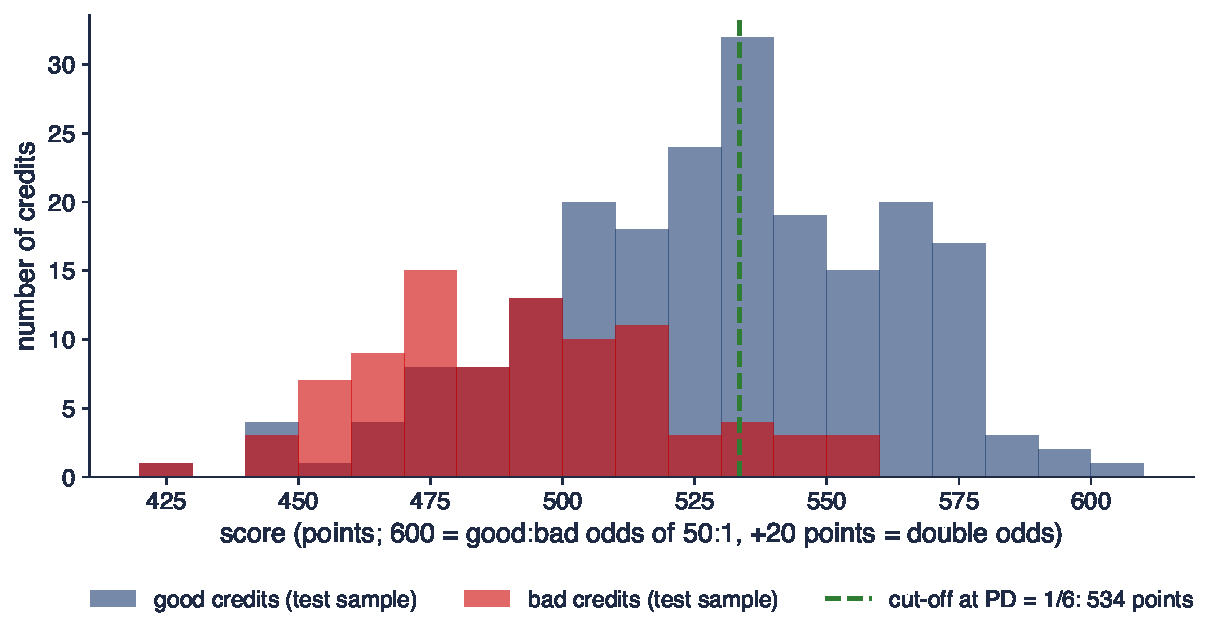
\includegraphics[width=0.97\textwidth,height=0.50\textheight,keepaspectratio]{sfm_ch12_score_dist.pdf}
\end{center}
\vspace{-0.25cm}
\begin{itemize}
    \item 300 de credite de test; scoruri de la 422 la 607 de puncte; media: bun-platnici 529, rău-platnici 492; linia întreruptă: pragul la PD $= 1/6$ (secțiunea 7), 534 de puncte
    \item Interpretare: cele două distribuții sînt deplasate, dar se suprapun: orice prag respinge unii bun-platnici și acceptă unii rău-platnici; măsurile de validare cuantifică această suprapunere
\end{itemize}
\sfmquantlet{Ch_12}{SFM_ch12_scorecard}
\end{frame}


%=============================================================================
\section{Validarea}
%=============================================================================

\begin{frame}{Matricea de confuzie}
\itemsize{\footnotesize}
\begin{columns}[T]
\begin{column}{0.50\textwidth}
\begin{center}
\scriptsize
\begin{tabular}{lcc}
\toprule
& prezis rău (respins) & prezis bun (acceptat) \\
\midrule
rău-platnic real & TP & FN \\
bun-platnic real & FP & TN \\
\bottomrule
\end{tabular}
\end{center}

\end{column}
\begin{column}{0.48\textwidth}
\begin{itemize}
    \item Un prag $c$: respingem dacă PD $> c$
    \item TP (true positive): un rău-platnic respins; FN (false negative): un rău-platnic acceptat
    \item FP (false positive): un bun-platnic respins; TN (true negative): un bun-platnic acceptat
\end{itemize}
\end{column}
\end{columns}\begin{itemize}
    \item Ratele
    \begin{itemize}
        \item \textbf{TPR} (true positive rate, sensibilitatea) $= \mathrm{TP}/(\mathrm{TP} + \mathrm{FN})$: ponderea rău-platnicilor identificați
        \item \textbf{FPR} (false positive rate) $= \mathrm{FP}/(\mathrm{FP} + \mathrm{TN}) = 1 -$ specificitatea: ponderea bun-platnicilor respinși
        \item precizia $= \mathrm{TP}/(\mathrm{TP} + \mathrm{FP})$; acuratețea $= (\mathrm{TP} + \mathrm{TN})/n$
    \end{itemize}
    \item Fiecare rată depinde de $c$; măsurile următoare rezumă toate pragurile deodată
\end{itemize}
\end{frame}

\begin{frame}{Două praguri pe eșantionul de test}
\itemsize{\footnotesize}
\begin{center}
\scriptsize
\begin{tabular}{lrrrrrrrr}
\toprule
prag & TP & FN & FP & TN & acuratețe & TPR & FPR & cost \\
\midrule
PD $> 0{,}5$ & 43 & 47 & 25 & 185 & $76{,}0\%$ & $47{,}8\%$ & $11{,}9\%$ & $0{,}867$ \\
PD $> 1/6$ & 82 & 8 & 112 & 98 & $60{,}0\%$ & $91{,}1\%$ & $53{,}3\%$ & $0{,}507$ \\
\bottomrule
\end{tabular}
\end{center}
\begin{itemize}
    \item Costul pe solicitant $= (5\,\mathrm{FN} + 1\,\mathrm{FP})/n$: acceptarea unui rău-platnic costă de cinci ori mai mult decît respingerea unui bun-platnic \refGroemping
    \begin{itemize}
        \item pragul Bayes minimizează costul așteptat: respingem dacă $p\,C_{FN} > (1 - p)\,C_{FP}$, adică $p > C_{FP}/(C_{FP} + C_{FN}) = 1/6$
    \end{itemize}
    \item Interpretare: pragul de 1/6 are o acuratețe mai mică (60{,}0\% față de 76{,}0\%), dar un cost mult mai mic (0{,}507 față de 0{,}867): identifică 91{,}1\% din rău-platnici
\end{itemize}\sfmquantlet{Ch_12}{SFM_ch12_validation_irb}
\end{frame}

\begin{frame}{Costul așteptat și alegerea pragului}
\itemsize{\footnotesize}
\begin{center}
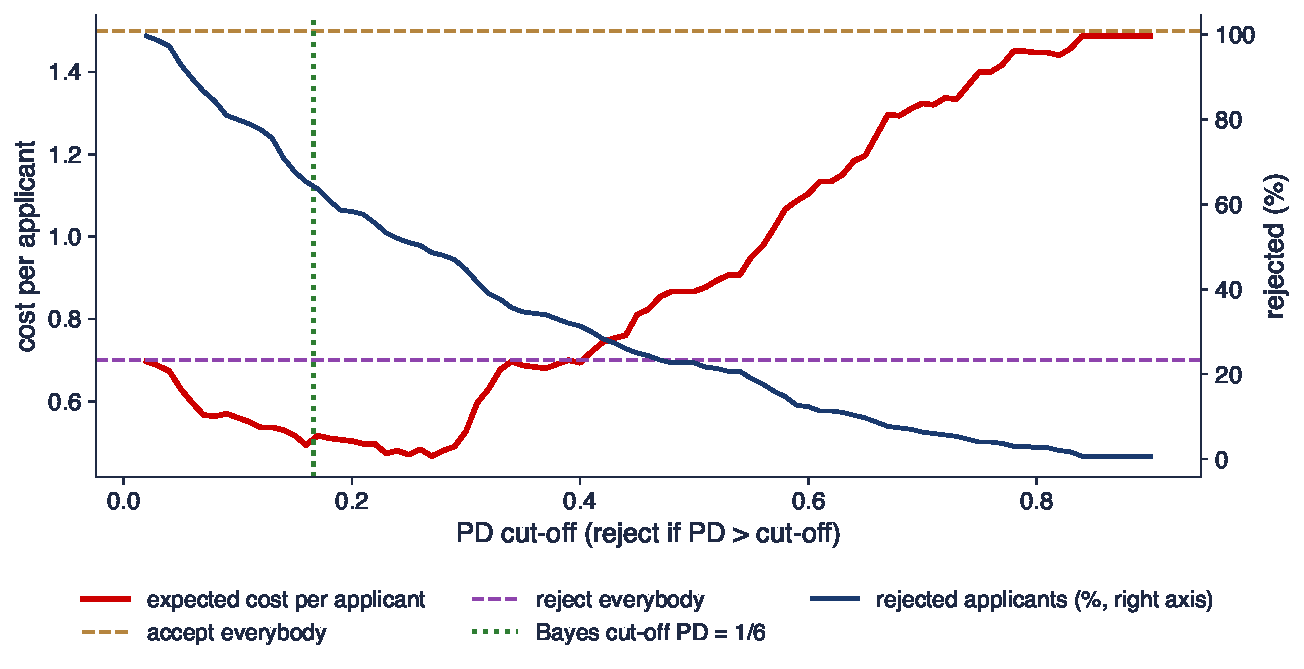
\includegraphics[width=0.97\textwidth,height=0.50\textheight,keepaspectratio]{sfm_ch12_cost_cutoff.pdf}
\end{center}
\vspace{-0.25cm}
\begin{itemize}
    \item Eșantionul de test; roșu: costul pe solicitant; linii întrerupte: acceptăm pe toată lumea (1{,}50) sau respingem pe toată lumea (0{,}70); albastru: ponderea respinșilor (axa din dreapta)
    \item Interpretare: costul este aproape constant între PD 0,1 și 0,3; minimul pe aceste 300 de credite este la 0{,}27, aproape de pragul Bayes de 1/6, care se alege înainte de a vedea datele de test
\end{itemize}
\sfmquantlet{Ch_12}{SFM_ch12_validation_irb}
\end{frame}

\begin{frame}{Curba ROC și AUC}
\itemsize{\small}
\begin{itemize}
    \item \textbf{ROC} (receiver operating characteristic): punctele (FPR$(c)$, TPR$(c)$) pentru toate pragurile $c$
    \begin{itemize}
        \item de la (0, 0) (nu respingem pe nimeni) la (1, 1) (respingem pe toată lumea); diagonala este un scor aleator
    \end{itemize}
    \item \textbf{AUC} (aria de sub curbă) $= P(s_{\text{rău}} > s_{\text{bun}}) + \tfrac12 P(s_{\text{rău}} = s_{\text{bun}})$ \refHM
    \begin{itemize}
        \item $s$: scorul de risc (aici PD); se calculează numărînd perechile: ponderea perechilor (rău, bun) ordonate corect
        \item statistica Mann--Whitney împărțită la $n_1 n_0$; 0,5: nicio discriminare, 1: perfectă
    \end{itemize}
    \item \textbf{Gini} $= 2\,\mathrm{AUC} - 1$; AUC nu depinde de rata rău-platnicilor sau de o transformare monotonă a scorului
    \begin{itemize}
        \item eroarea standard și testele pentru AUC: \refDeLong
    \end{itemize}
\end{itemize}
\end{frame}

\begin{frame}{Curbele ROC pe eșantionul de test}
\itemsize{\footnotesize}
\begin{columns}[T]
\begin{column}{0.47\textwidth}
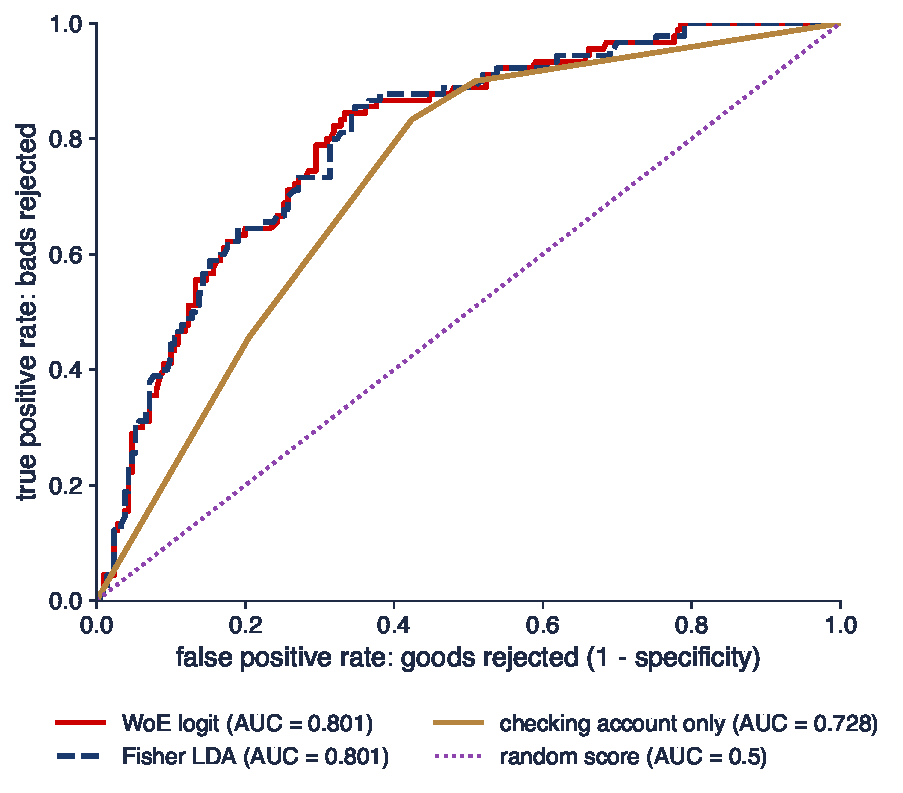
\includegraphics[width=\textwidth,height=0.64\textheight,keepaspectratio]{sfm_ch12_roc.pdf}
\end{column}
\begin{column}{0.51\textwidth}
\begin{itemize}
    \item 300 de credite de test, 18\,900 de perechi (rău, bun)
    \item Logit WoE: AUC $= 0{,}801$, CI 95\% $[0{,}749; 0{,}854]$ (DeLong, se $0{,}027$); Gini $= 0{,}603$
    \item Doar contul curent: AUC $= 0{,}728$; testul DeLong față de scorecard: $z = 2{,}86$, p $= 0{,}004$
    \item Interpretare: un rău-platnic ales la întîmplare are o PD mai mare decît un bun-platnic ales la întîmplare în aproximativ 80\% din perechi; celelalte cinci variabile aduc o îmbunătățire semnificativă față de contul curent
\end{itemize}
\end{column}
\end{columns}
\sfmquantlet{Ch_12}{SFM_ch12_validation_irb}
\end{frame}

\begin{frame}{Curba CAP, raportul de acuratețe și KS}
\itemsize{\small}
\begin{itemize}
    \item \textbf{CAP} (cumulative accuracy profile): ordonăm solicitanții de la cel mai riscant; reprezentăm ponderea tuturor rău-platnicilor printre primii $x\%$
    \begin{itemize}
        \item modelul perfect: toți rău-platnicii primii, curba atinge 1 la $x = $ rata rău-platnicilor; aleator: diagonala
        \item \textbf{AR} (accuracy ratio, raportul de acuratețe) $= \dfrac{\text{aria dintre CAP-ul modelului și diagonală}}{\text{aria dintre CAP-ul perfect și diagonală}}$; pentru un scor continuu AR $=$ Gini
    \end{itemize}
    \item \textbf{KS} (Kolmogorov--Smirnov): $\max_s |F_{\text{rău}}(s) - F_{\text{bun}}(s)|$, cea mai mare distanță dintre distribuțiile scorurilor rău-platnicilor și bun-platnicilor
    \begin{itemize}
        \item $F_{\text{rău}}$, $F_{\text{bun}}$: funcțiile de repartiție empirice ale scorurilor în cele două grupuri; KS $\in [0, 1]$
        \item citit pe curba ROC: KS $= \max_c\,(\mathrm{TPR} - \mathrm{FPR})$; scorul la care apare este un prim prag natural
    \end{itemize}
    \item Toate cele trei măsoară \textbf{discriminarea} (ordonarea), nu calibrarea
\end{itemize}
\end{frame}

\begin{frame}{CAP și KS pe eșantionul de test}
\itemsize{\footnotesize}
\begin{columns}[T]
\begin{column}{0.44\textwidth}
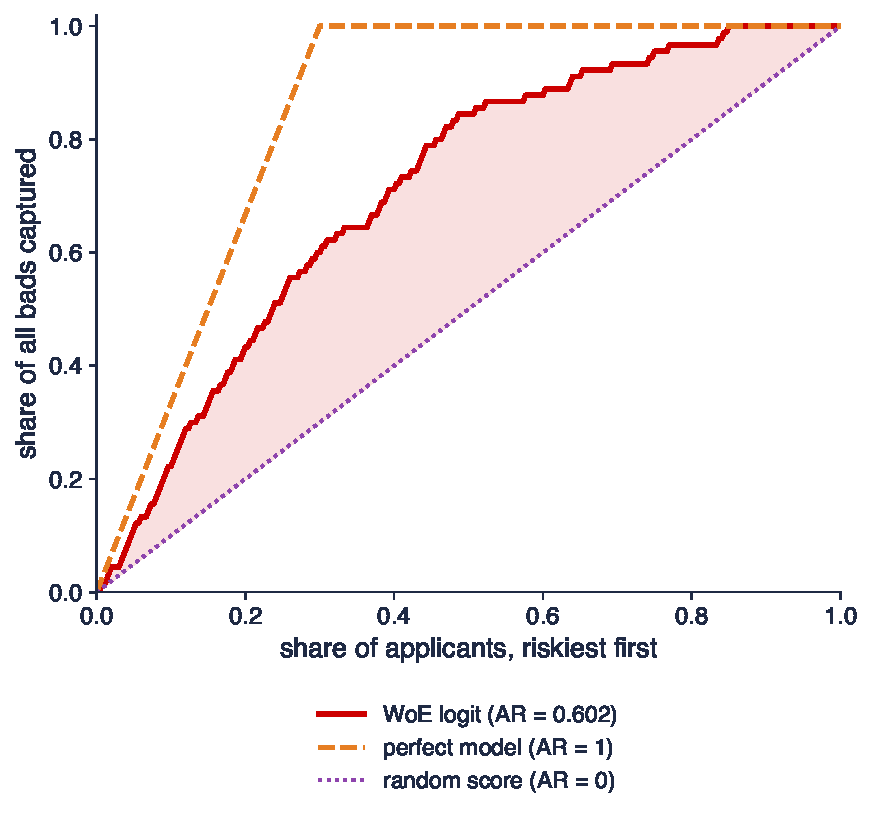
\includegraphics[width=\textwidth,height=0.50\textheight,keepaspectratio]{sfm_ch12_cap.pdf}
\end{column}
\begin{column}{0.54\textwidth}
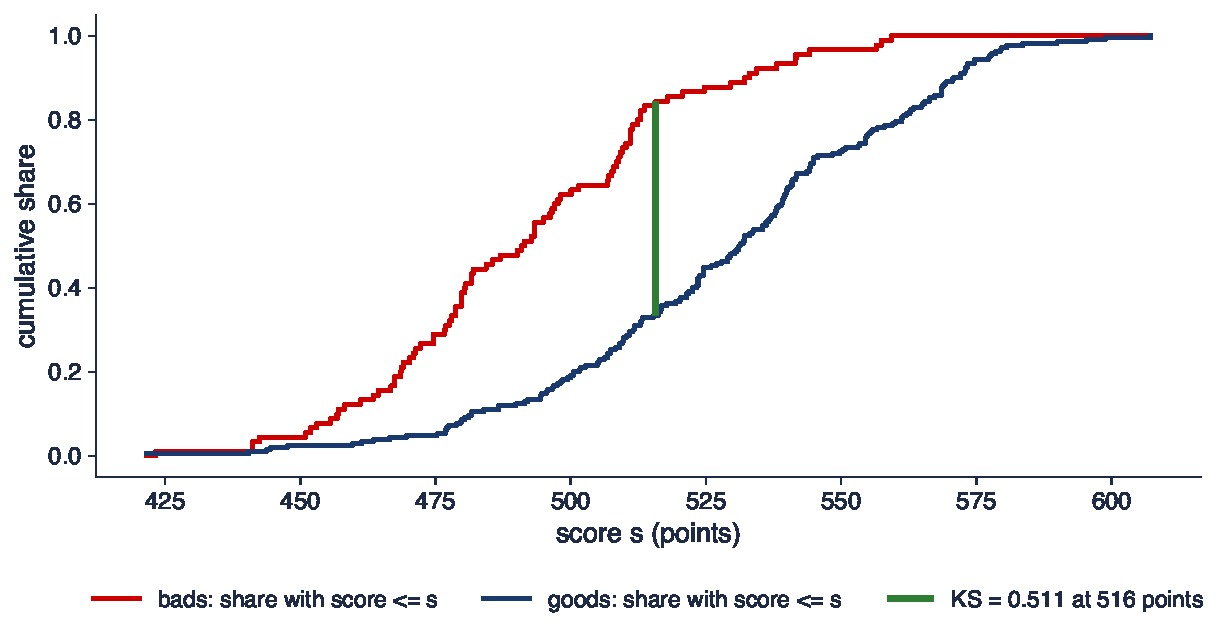
\includegraphics[width=\textwidth,height=0.50\textheight,keepaspectratio]{sfm_ch12_ks.pdf}
\end{column}
\end{columns}\begin{itemize}
    \item AR $= 0{,}602$ (Gini $= 0{,}603$: același, cu excepția rotunjirii); KS $= 0{,}511$ la 516 de puncte
    \item Interpretare: respingînd cei mai riscanți 30\%, identificăm aproximativ două treimi din rău-platnici; la 516 de puncte, scorecard-ul separă cel mai bine rău-platnicii de bun-platnici
\end{itemize}\sfmquantlet{Ch_12}{SFM_ch12_validation_irb}
\end{frame}

\begin{frame}{Calibrarea și scorul Brier}
\itemsize{\small}
\begin{itemize}
    \item \textbf{Calibrarea}: dintre solicitanții cu PD $\approx p$, aproximativ o pondere $p$ intră în nerambursare
    \begin{itemize}
        \item diagrama de calibrare: ordonăm după PD, formăm grupuri (de exemplu zece), reprezentăm PD medie față de rata observată
        \item Hosmer--Lemeshow \refHL: $\sum_g \dfrac{(O_g - n_g\bar p_g)^2}{n_g\bar p_g(1 - \bar p_g)} \approx \chi^2(G - 2)$
        \item $G$ grupuri; $n_g$: mărimea, $O_g$: nerambursările observate, $\bar p_g$: PD medie a grupului $g$; o valoare mare: calibrare slabă
    \end{itemize}
    \item \textbf{Scorul Brier} \refBrier: $\mathrm{BS} = \frac1n\sum_i (p_i - y_i)^2$, eroarea pătratică medie a PD; o valoare mai mică este mai bună
    \begin{itemize}
        \item referința: o PD constantă egală cu rata din eșantionul de estimare; cîștigul $= 1 - \mathrm{BS}/\mathrm{BS}_{\text{ref}}$
        \item eșantionul de test al scorecard-ului: BS $= 0{,}162$ față de $0{,}210$ (cîștig 23\%); HL cu 10 grupuri $= 6{,}520$, p $= 0{,}589$
    \end{itemize}
    \item Scorul Brier recompensează atît ordonarea, cît și calibrarea; AUC măsoară doar ordonarea
\end{itemize}
\end{frame}

\begin{frame}{Calibrarea pe datele din Taiwan}
\itemsize{\footnotesize}
\begin{columns}[T]
\begin{column}{0.44\textwidth}
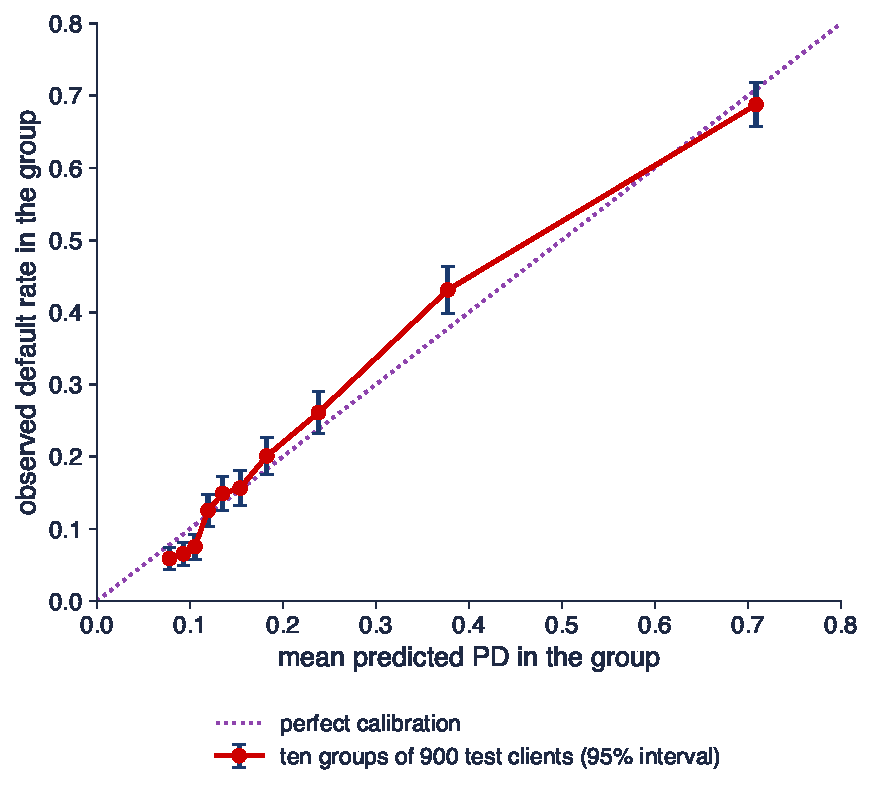
\includegraphics[width=\textwidth,height=0.62\textheight,keepaspectratio]{sfm_ch12_calibration.pdf}
\end{column}
\begin{column}{0.54\textwidth}
\begin{itemize}
    \item Logit pe 30\,000 de deținători de card (70\% estimare); eșantion de test de 9\,000; zece grupuri de cîte 900 după PD; bare: intervale de 95\%
    \item AUC de test $= 0{,}777$ (estimare $0{,}774$); Brier $= 0{,}136$ față de $0{,}172$ (cîștig 21\%)
    \item Hosmer--Lemeshow $= 40{,}660$, p $<$\,0{,}001: respins, deși punctele sînt aproape de diagonală
    \item Interpretare: cu 9000 de clienți, testul detectează abateri mici (grupul cel mai sigur: PD 7{,}8\%, observat 5{,}9\%); judecăm mărimea abaterilor, nu doar p-value-ul
\end{itemize}
\end{column}
\end{columns}
\sfmquantlet{Ch_12}{SFM_ch12_validation_irb}
\end{frame}

\begin{frame}{Validarea în afara eșantionului și validarea încrucișată}
\itemsize{\small}
\begin{itemize}
    \item Performanța \textbf{în eșantion} este optimistă: modelul s-a adaptat la zgomotul datelor de estimare (supraajustare)
    \begin{itemize}
        \item un eșantion de test de 300 de credite dă AUC $= 0{,}801$ cu o eroare standard de $0{,}027$: o singură împărțire este zgomotoasă
    \end{itemize}
    \item \textbf{Validarea încrucișată în $k$ părți}: împărțim în $k = 5$ părți; estimăm pe patru, testăm pe a cincea; rotim; repetăm de 20 de ori
    \begin{itemize}
        \item întreaga procedură se repetă în fiecare parte: intervale, WoE, selecția după IV și coeficienții
        \item raportăm media și dispersia celor 100 de AUC de test, precum și diferența dintre AUC de estimare și de test
    \end{itemize}
    \item Validarea \textbf{out-of-time}: estimăm pe cereri mai vechi, testăm pe cereri ulterioare (slide-ul următor)
\end{itemize}
\end{frame}

\begin{frame}{AUC de estimare și de test în validarea încrucișată repetată}
\itemsize{\footnotesize}
\begin{center}
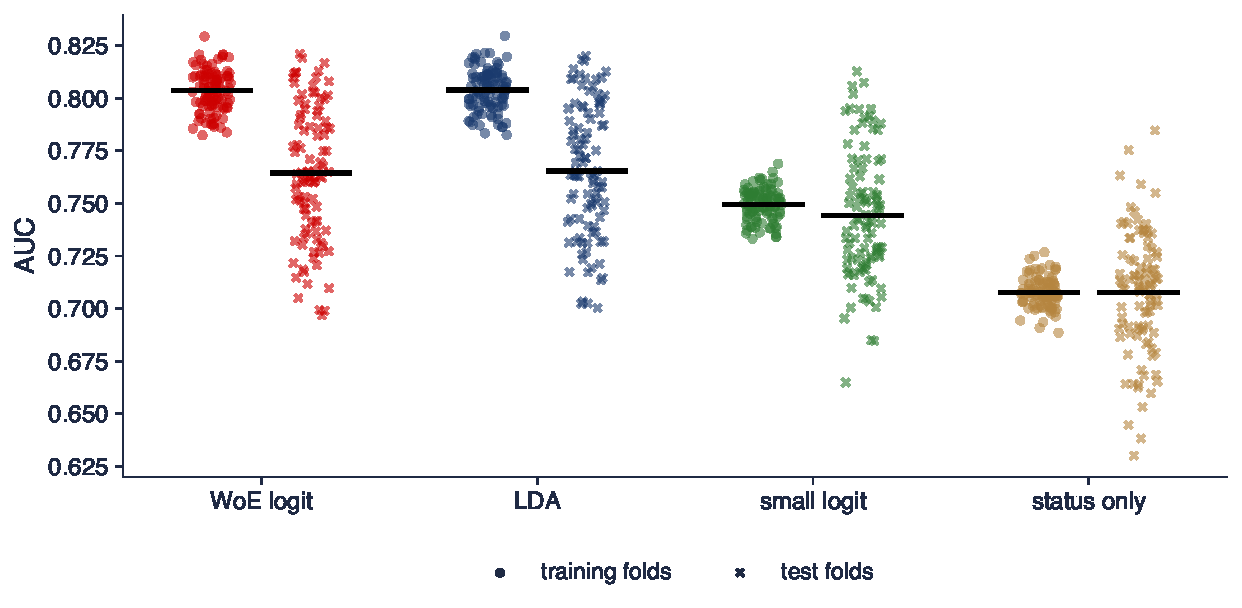
\includegraphics[width=0.97\textwidth,height=0.46\textheight,keepaspectratio]{sfm_ch12_cv_auc.pdf}
\end{center}
\vspace{-0.25cm}
\begin{itemize}
    \item 20 de repetări a cîte 5 părți; puncte: părțile de estimare, cruci: părțile de test; liniile negre: mediile
    \item Logit WoE: estimare $0{,}804$, test $0{,}764$ (sd $0{,}032$); LDA: $0{,}804$, $0{,}765$; logit mic: $0{,}749$, $0{,}744$; contul curent: $0{,}708$
    \item Interpretare: scorecard-ul pierde 0{,}039 din AUC în afara eșantionului, logit-ul cu cinci variabile aproape nimic; împărțirea unică de mai sus a fost norocoasă ($0{,}801$ față de $0{,}764$ în medie)
\end{itemize}
\sfmquantlet{Ch_12}{SFM_ch12_validation_irb}
\end{frame}

\begin{frame}{Validarea out-of-time și deriva populației}
\itemsize{\small}
\begin{itemize}
    \item Un scorecard este folosit ani de zile pe solicitanți care vin \textbf{după} perioada de estimare
    \begin{itemize}
        \item economia, produsele și solicitanții se schimbă: relația dintre $x$ și nerambursare se modifică în timp
        \item testul out-of-time: estimăm, de exemplu, pe 2019--2021, testăm pe 2022--2023; comparăm AUC și calibrarea de la un an la altul
    \end{itemize}
    \item Monitorizarea: distribuția scorurilor și a fiecărei variabile se compară cu perioada de estimare
    \begin{itemize}
        \item o deplasare cu ordonare stabilă cere recalibrare (termenul liber); o pierdere a ordonării cere un model nou
    \end{itemize}
    \item Limitarea datelor: niciunul dintre seturile de date ale capitolului nu conține data cererilor, deci un test out-of-time nu este posibil aici; putem folosi doar împărțiri aleatoare
    \item Lectură suplimentară despre un design out-of-time, pentru activele cripto „zombie”: \refPeleZ
\end{itemize}
\end{frame}

\begin{frame}{Studiu de caz: compararea metodelor de scoring}
\itemsize{\small}
\begin{itemize}
    \item \refLessmann: 41 de clasificatori, șase măsuri de acuratețe, opt seturi de date de retail (printre ele datele germane de credit din UCI)
    \begin{itemize}
        \item o actualizare, după zece ani, a comparației lui Baesens et al.\ (2003)
    \end{itemize}
    \item Rezultatele
    \begin{itemize}
        \item mai mulți clasificatori prezic semnificativ mai bine decît regresia logistică, standardul industriei; ansamblurile eterogene sînt cele mai bune
        \item scorecard-urile mai precise pot aduce cîștiguri financiare importante
        \item măsurile uzuale de acuratețe dau semnale asemănătoare; random forests sînt recomandate ca reper pentru orice metodă nouă
    \end{itemize}
    \item A învinge doar logit-ul nu mai este o dovadă de progres; pe cele 1000 de credite, logit și LDA diferă cu mai puțin de o eroare standard a AUC; \sfmchlink{https://danpele.github.io/SFM/RO/Cursuri/capitol13_invatare_automata.pdf}{Capitolul 13} adaugă arbori și rețele neuronale
\end{itemize}
\end{frame}

\begin{frame}{Recapitulare: validarea}
\itemsize{\small}
\begin{itemize}
    \item Discriminarea: ROC, AUC, Gini $=$ AR, KS; calibrarea: diagrama de calibrare, Hosmer--Lemeshow, scorul Brier
    \item Alegem pragul din costuri, nu din acuratețe
    \item Testăm în afara eșantionului, repetăm cu validarea încrucișată și testăm out-of-time ori de cîte ori setul de date conține data cererilor
\end{itemize}
\end{frame}


%=============================================================================
\section{Reject inference și echitatea}
%=============================================================================

\begin{frame}{Reject inference}
\itemsize{\small}
\begin{itemize}
    \item Rezultatul este cunoscut doar pentru solicitanții \textbf{acceptați}; modelul se folosește pe \textbf{toți} solicitanții („through the door”)
    \begin{itemize}
        \item un eșantion selectat de scorul vechi: lipsesc solicitanții cei mai riscanți și rezultatele lor
        \item debitorii din South German Credit trecuseră toți de verificările băncii \refGroemping
    \end{itemize}
    \item \textbf{Reject inference}: metode care încearcă să corecteze lipsa rezultatelor \refBCT; \refTCE
    \begin{itemize}
        \item reponderarea: dăm o pondere mai mare acceptaților care seamănă cu respinșii
        \item augmentarea și parcelarea: atribuim rezultate respinșilor pe baza unui model
        \item sursa cea mai fiabilă: un mic eșantion aleator de solicitanți acceptați indiferent de scor
    \end{itemize}
\end{itemize}
\end{frame}

\begin{frame}{Un experiment de reject inference pe datele din Taiwan}
\itemsize{\footnotesize}
\begin{itemize}
    \item Un „scor vechi” (întîrzierea din septembrie și limita) acceptă cei mai buni 70\% dintre clienții de estimare (15\,085); rata lor de nerambursare este 13{,}2\%, a respinșilor 44{,}9\%
    \begin{itemize}
        \item printre acceptați nimeni nu a întîrziat în septembrie: variabila cea mai puternică nu poate fi estimată și iese din model
    \end{itemize}
    \item Eșantionul de test (toți solicitanții): AUC al modelului estimat doar pe acceptați $0{,}736$, al celui estimat pe toți $0{,}777$, al scorului vechi $0{,}743$
    \begin{itemize}
        \item clienții de test respinși: rata observată 46{,}1\%; PD medie a modelului estimat pe acceptați 29{,}6\%, a modelului complet 44{,}1\%
    \end{itemize}
    \item Interpretare: estimat doar pe acceptați, noul model ordonează mai slab decît scorul vechi și subestimează riscul respinșilor cu aproximativ 36\%
\end{itemize}\sfmquantlet{Ch_12}{SFM_ch12_reject_fairness}
\end{frame}

\begin{frame}{Echitatea (fairness) în scoringul de credit}
\itemsize{\footnotesize}
\begin{columns}[T]
\begin{column}{0.62\textwidth}
\begin{itemize}
    \item Legea americană interzice discriminarea în creditare după sex, stare civilă, rasă, religie, origine națională sau vîrstă \refECOA
    \begin{itemize}
        \item UE: scoringul de credit al persoanelor este o utilizare cu risc ridicat a AI (documentare, supraveghere umană) \refAIAct
    \end{itemize}
    \item Excluderea variabilei protejate nu este suficientă: alte variabile o pot înlocui
    \begin{itemize}
        \item \textbf{paritatea demografică}: rate egale de aprobare între grupuri
        \item \textbf{egalitatea de șanse}: rate egale de aprobare pentru bun-platnici \refHPS
        \item \textbf{calibrarea în fiecare grup}: aceeași PD înseamnă același risc în fiecare grup
    \end{itemize}
    \item Cînd ratele de nerambursare diferă între grupuri, aceste criterii nu pot fi toate îndeplinite simultan: alegerea ține de politica băncii și a autorităților
\end{itemize}
\end{column}
\begin{column}{0.35\textwidth}
\centering
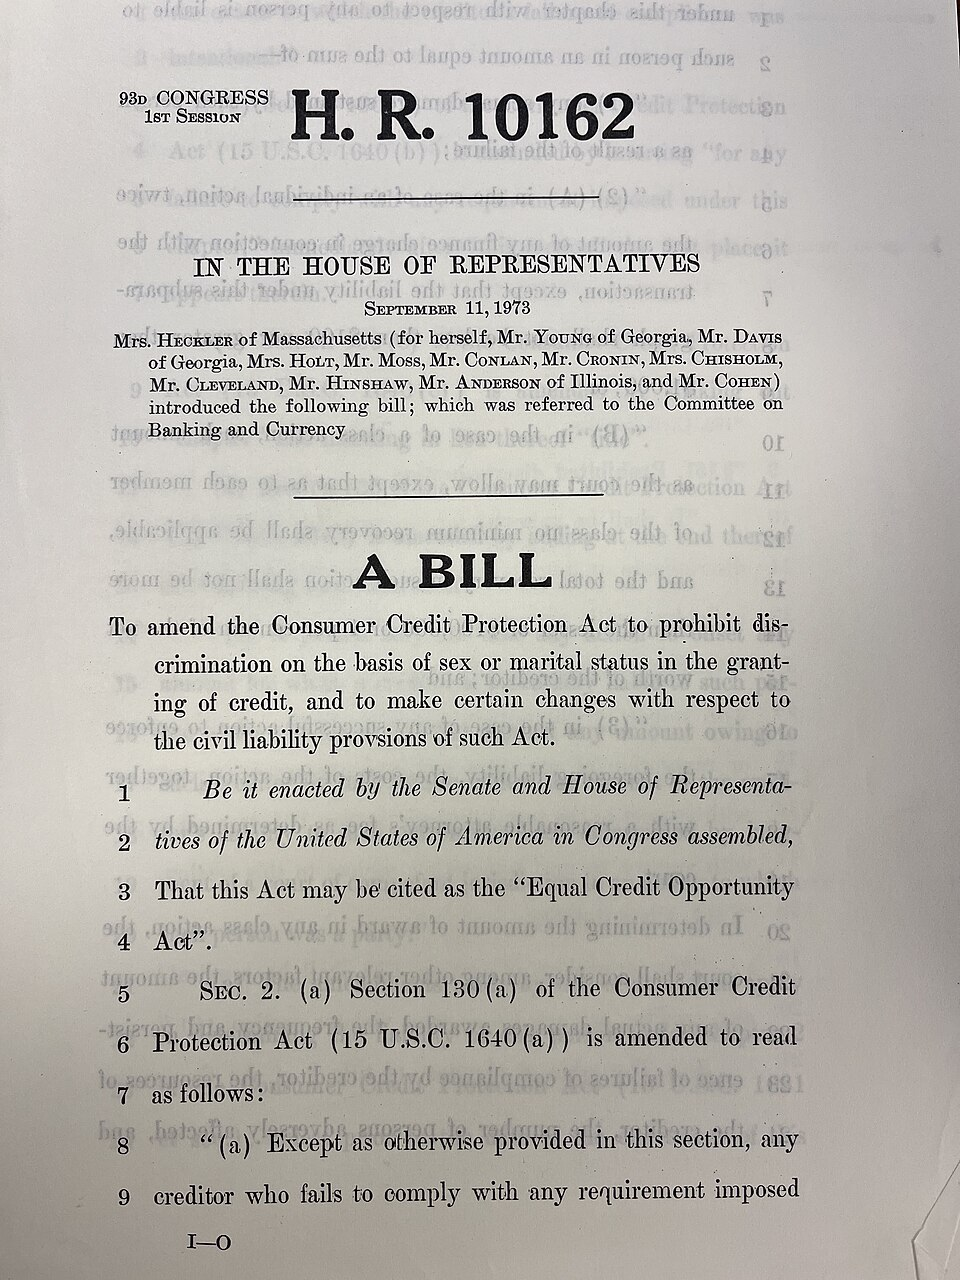
\includegraphics[height=0.46\textheight]{ch12_heckler_bill_1973.jpg}\\[1mm]
\imgcap{H.R. 10162 (1973), proiectul de lege care a introdus Equal Credit Opportunity Act}
\imgcredit{https://commons.wikimedia.org/wiki/File:A_Bill_to_amend_the_Consumer_Credit_Protection_Act.jpg}{Foto: H.R. 10162 (1973); domeniu public; Wikimedia Commons}
\end{column}
\end{columns}
\end{frame}

\begin{frame}{Aprobarea și nerambursarea pe grupuri: Taiwan}
\itemsize{\footnotesize}
\begin{center}
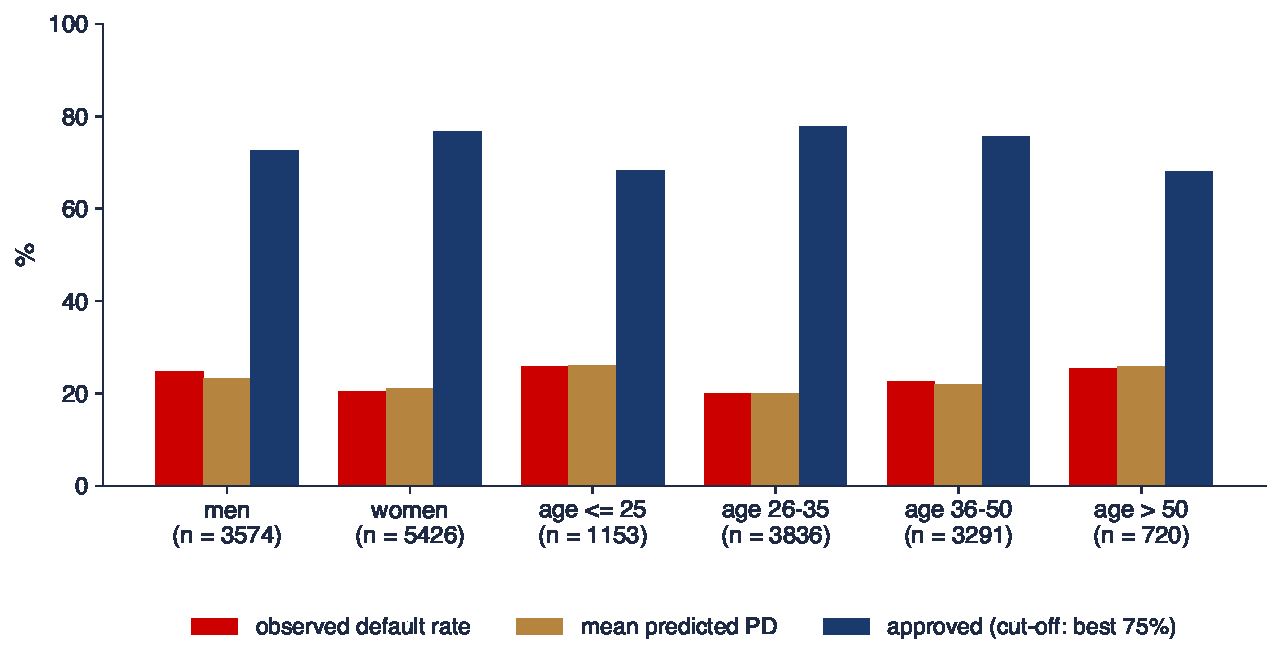
\includegraphics[width=0.97\textwidth,height=0.46\textheight,keepaspectratio]{sfm_ch12_fairness.pdf}
\end{center}
\vspace{-0.25cm}
\begin{itemize}
    \item Eșantionul de test; sexul și vîrsta nu sînt variabile ale modelului; pragul: aprobăm cei 75\% cu PD cea mai mică
    \item Femei: rata de nerambursare 20{,}5\%, aprobate 76{,}6\%; bărbați: 24{,}7\%, 72{,}5\%; bun-platnici aprobați: femei 85{,}1\%, bărbați 83{,}2\%
    \item Interpretare: modelul este calibrat în fiecare grup (PD medie apropiată de rata observată), deci grupurile cu mai multe nerambursări (bărbații, cei mai tineri și cei mai în vîrstă) sînt aprobate mai rar
\end{itemize}
\sfmquantlet{Ch_12}{SFM_ch12_reject_fairness}
\end{frame}

\begin{frame}{Studiu de caz: învățarea automată și creditul inegal}
\itemsize{\small}
\begin{itemize}
    \item \refFuster: credite ipotecare din SUA; nerambursarea prezisă cu un logit tradițional și cu modele de învățare automată
    \begin{itemize}
        \item întrebarea: cine cîștigă și cine pierde cînd creditorul trece la modelul mai precis?
    \end{itemize}
    \item Rezultatele
    \begin{itemize}
        \item modelele flexibile prezic mai bine nerambursarea
        \item debitorii de culoare și cei hispanici au mai puține șanse să cîștige din noua tehnologie
        \item într-un model de echilibru, disparitatea dobînzilor între grupuri și în interiorul lor crește, mai ales din cauza flexibilității mai mari
    \end{itemize}
    \item Lecția: acuratețea și echitatea trebuie măsurate împreună; un AUC mai bun nu este un argument suficient
\end{itemize}
\end{frame}

\begin{frame}{Recapitulare: reject inference și echitatea}
\itemsize{\small}
\begin{itemize}
    \item Rezultatele există doar pentru solicitanții acceptați: un model estimat pe ei extrapolează la cei respinși
    \item Criteriile de echitate (paritate, egalitate de șanse, calibrare) intră în conflict cînd ratele de bază diferă
    \item Eliminarea unei variabile protejate nu îi elimină influența
\end{itemize}
\end{frame}


%=============================================================================
\section{Nerambursarea companiilor: Altman și Merton}
%=============================================================================

\begin{frame}{Scorul Z al lui Altman (1968)}
\itemsize{\footnotesize}
\begin{columns}[T]
\begin{column}{0.60\textwidth}
\begin{itemize}
    \item \refAltman: 66 de companii industriale americane, 33 care au intrat în faliment în 1946--1965 și 33 de companii pereche care au supraviețuit
    \begin{itemize}
        \item analiza discriminantă a lui Fisher pe cinci indicatori contabili
    \end{itemize}
    \item $Z = 1{,}2X_1 + 1{,}4X_2 + 3{,}3X_3 + 0{,}6X_4 + 1{,}0X_5$
    \begin{itemize}
        \item $X_1$ capitalul de lucru / activele totale (TA); $X_2$ profitul reinvestit / TA; $X_3$ EBIT (profitul înainte de dobînzi și impozite) / TA
        \item $X_4$ valoarea de piață a capitalurilor proprii / valoarea contabilă a datoriilor; $X_5$ cifra de afaceri / TA
        \item zonele: $Z < 1{,}81$ dificultate, $1{,}81$--$2{,}99$ zona gri, $Z > 2{,}99$ sigur
    \end{itemize}
    \item Aproximativ 95\% din eșantion clasificat corect cu un an înainte de faliment; acuratețea scade repede pentru orizonturi mai lungi
\end{itemize}
\end{column}
\begin{column}{0.37\textwidth}
\centering
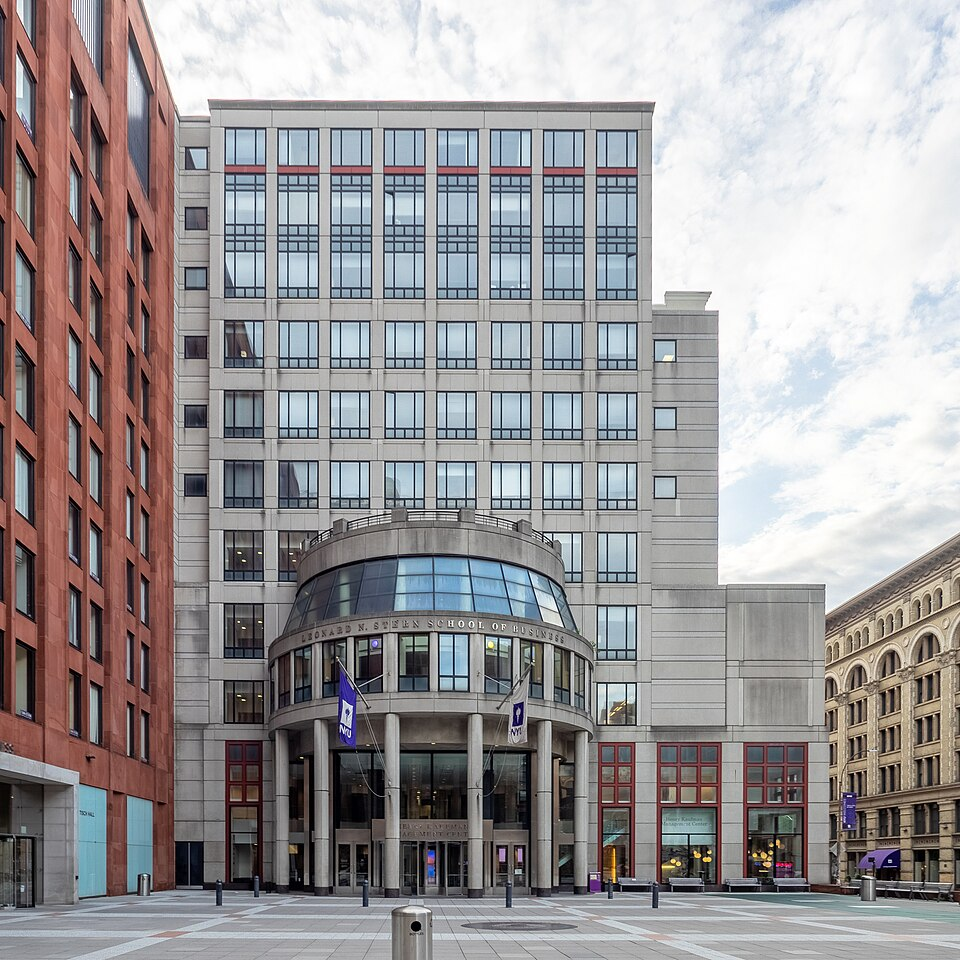
\includegraphics[height=0.36\textheight]{ch12_nyu_stern_2019.jpg}\\[1mm]
\imgcap{NYU Stern School of Business, instituția lui Altman}
\imgcredit{https://commons.wikimedia.org/wiki/File:NYU_Stern_School_of_Business_-_Henry_Kaufman_Management_Center_(48072761732).jpg}{Foto: Ajay Suresh (2019); CC BY 2.0; Wikimedia Commons}
\end{column}
\end{columns}
\end{frame}

\begin{frame}{Exemplu rezolvat: un scor Z}
\itemsize{\small}
\begin{itemize}
    \item O companie ipotetică: $X_1 = 0{,}15$, $X_2 = 0{,}20$, $X_3 = 0{,}08$, $X_4 = 0{,}90$, $X_5 = 1{,}10$
    \begin{itemize}
        \item $Z = 1{,}2 \times 0{,}15 + 1{,}4 \times 0{,}20 + 3{,}3 \times 0{,}08 + 0{,}6 \times 0{,}90 + 1{,}0 \times 1{,}10$
        \item $Z = 0{,}180 + 0{,}280 + 0{,}264 + 0{,}540 + 1{,}100 = 2{,}364$: zona gri
    \end{itemize}
    \item Ce indicator ar muta compania în zona sigură?
    \begin{itemize}
        \item un EBIT/TA de 0,27 în loc de 0,08 adaugă $3{,}3 \times 0{,}19 \approx 0{,}63$: $Z \approx 2{,}99$
    \end{itemize}
    \item Limite
    \begin{itemize}
        \item ponderile provin din 66 de companii industriale americane din 1946--1965; alte sectoare și țări cer reestimare
        \item Z este un scor discriminant, nu o PD; modelele ulterioare dau PD: logit \refOhlson, modele de hazard \refShumway
    \end{itemize}
\end{itemize}
\end{frame}

\begin{frame}{Distanța pînă la nerambursare a lui Merton}
\itemsize{\footnotesize}
\begin{columns}[T]
\begin{column}{0.66\textwidth}
\begin{itemize}
    \item \refMerton: valoarea $V_t$ a activelor companiei urmează o GBM (mișcarea browniană geometrică, \sfmchlink{https://danpele.github.io/SFM/RO/Cursuri/capitol4_probabilitate.pdf}{Capitolul 4}) cu rata de creștere (drift) $\mu$ și volatilitatea $\sigma_V$
    \begin{itemize}
        \item datorie cu valoarea nominală $D$ scadentă la $T$; nerambursare dacă $V_T < D$; capitalurile proprii sînt o opțiune call pe active
    \end{itemize}
    \item $\ln V_T \sim N\big(\ln V_0 + (\mu - \sigma_V^2/2)T,\ \sigma_V^2T\big)$, deci
    \begin{itemize}
        \item $\mathrm{DD} = \dfrac{\ln(V_0/D) + (\mu - \sigma_V^2/2)T}{\sigma_V\sqrt{T}}$, \quad $\mathrm{PD} = \Phi(-\mathrm{DD})$
        \item DD: numărul de abateri standard dintre valoarea așteptată a activelor și datorie
    \end{itemize}
    \item $V$ și $\sigma_V$ nu sînt observabile: se obțin din prețul și volatilitatea acțiunilor (evaluarea opțiunilor)
\end{itemize}
\end{column}
\begin{column}{0.31\textwidth}
\centering

\includegraphics[height=0.42\textheight]{ch12_merton_2010.jpg}\\[1mm]
\imgcap{Robert C. Merton, 2010}
\imgcredit{https://commons.wikimedia.org/wiki/File:Robert_Merton_November_2010_(2x3_cropped).jpg}{Foto: Massachusetts Institute of Technology (2010); CC BY-SA 4.0; Wikimedia Commons}
\end{column}
\end{columns}
\end{frame}

\begin{frame}{Exemplu rezolvat: distanța pînă la nerambursare}
\itemsize{\footnotesize}
\begin{itemize}
    \item $V_0 = 100$, $D = 70$, $\sigma_V = 25\%$, $\mu = 5\%$, $T = 1$ an
    \begin{itemize}
        \item $\ln(100/70) = 0{,}3567$; $\mu - \sigma_V^2/2 = 0{,}05 - 0{,}03125 = 0{,}01875$
        \item $\mathrm{DD} = 0{,}3754/0{,}25 = 1{,}502$; PD $= \Phi(-1{,}502) = 6{,}66\%$
    \end{itemize}
    \item Din piață: capitaluri proprii 40, volatilitatea acțiunilor 50\%, datorie 70, rata fără risc 3\%
    \begin{itemize}
        \item rezolvînd $E = V\Phi(d_1) - De^{-rT}\Phi(d_2)$ și $\sigma_E E = \Phi(d_1)\sigma_V V$: $V = 107{,}9$, $\sigma_V = 18{,}6\%$, DD $= 2{,}39$, PD $= 0{,}84\%$
        \item $E$, $\sigma_E$: valoarea și volatilitatea capitalurilor proprii; $r$: rata fără risc; $d_1$, $d_2$: termenii Black--Scholes din \sfmchlink{https://danpele.github.io/SFM/RO/Cursuri/capitol4_probabilitate.pdf}{Capitolul 4}, cu $V$ în locul prețului acțiunii
    \end{itemize}
    \item Interpretare: o PD din piață reacționează zilnic la prețuri; un scor contabil se schimbă o dată pe an
\end{itemize}\sfmquantlet{Ch_12}{SFM_ch12_altman_merton}
\end{frame}

\begin{frame}{Merton: traiectoriile activelor și PD}
\itemsize{\footnotesize}
\begin{center}
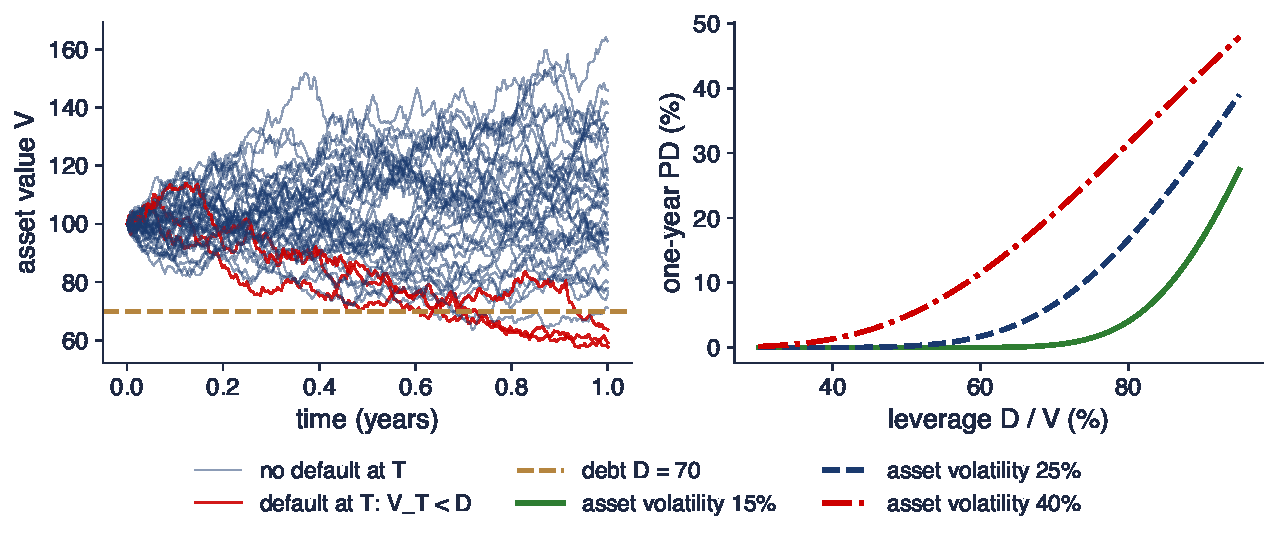
\includegraphics[width=0.97\textwidth,height=0.46\textheight,keepaspectratio]{sfm_ch12_merton.pdf}
\end{center}
\vspace{-0.25cm}
\begin{itemize}
    \item Stînga: 40 de traiectorii simulate ale activelor ($V_0 = 100$, $\mu = 5\%$, $\sigma_V = 25\%$); roșu: traiectoriile care se termină sub datoria de 70
    \item Dreapta: PD pe un an în funcție de gradul de îndatorare $D/V$ pentru trei volatilități ale activelor
    \item Interpretare: PD este aproape zero la îndatorare mică și crește abrupt între 70\% și 90\%; cu cît volatilitatea este mai mare, cu atît creșterea începe mai devreme
\end{itemize}
\sfmquantlet{Ch_12}{SFM_ch12_altman_merton}
\end{frame}

\begin{frame}{Studiu de caz: cît de bun este modelul Merton?}
\itemsize{\small}
\begin{itemize}
    \item \refBS: companii americane; DD Merton față de un DD „naiv”, cu aceeași formă funcțională, dar fără rezolvarea modelului
    \begin{itemize}
        \item designul: modele de hazard ale nerambursării și prognoze în afara eșantionului; comparație cu spread-urile CDS (credit default swap) și randamentele obligațiunilor
    \end{itemize}
    \item Rezultatele
    \begin{itemize}
        \item DD naiv funcționează puțin mai bine decît DD Merton în afara eșantionului
        \item alte variabile (de exemplu randamentele trecute) aduc informație: DD nu este o statistică suficientă pentru PD
        \item forma sa funcțională (îndatorarea raportată la volatilitate) este ceea ce îl face util
    \end{itemize}
    \item Lecția: teoria dă o variabilă bună, statistica decide cum o folosim; la fel pentru scorul Z
\end{itemize}
\end{frame}

\begin{frame}{Recapitulare: Altman și Merton}
\itemsize{\small}
\begin{itemize}
    \item Altman: LDA pe cinci indicatori contabili; pragurile 1,81 și 2,99
    \item Merton: capitalurile proprii sînt un call pe active; DD $= [\ln(V/D) + (\mu - \sigma^2/2)T]/(\sigma\sqrt{T})$, PD $= \Phi(-\mathrm{DD})$
    \item Ambele sînt folosite cel mai bine ca variabile ale unui model statistic de PD
\end{itemize}
\end{frame}


%=============================================================================
\section{AI pentru descoperire științifică}
%=============================================================================

\begin{frame}{O întrebare deschisă}
\itemsize{\small}
\begin{itemize}
    \item \textbf{Îmbunătățesc scorurile flexibile de învățare automată prognoza nerambursării suficient pentru a justifica pierderea de transparență și de echitate?}
    \begin{itemize}
        \item azi: logit-ul WoE și LDA ating un AUC de test de aproximativ 0{,}764; comparațiile găsesc cîștiguri semnificative pentru ansambluri \refLessmann
        \item cîștigurile pot fi inegale între grupuri \refFuster; mașini cu vectori suport pentru nerambursare: \refCHM
    \end{itemize}
    \item Întrebarea rămîne deschisă: cîștigurile depind de setul de date, de măsură și de populație; rezultatele solicitanților respinși nu se văd niciodată
    \item Instrumentele AI pot accelera un astfel de studiu; nu înlocuiesc verificarea lui \refWang
\end{itemize}
\end{frame}

\begin{frame}{Contribuția posibilă a AI}
\itemsize{\small}
\begin{itemize}
    \item \textbf{Literatura}: o listă a comparațiilor de metode de scoring și a studiilor despre echitatea creditării, cu seturile lor de date
    \item \textbf{Cod}: o primă versiune a unei comparații prin validare încrucișată a logit-ului WoE cu gradient boosting pe datele din Taiwan
    \item \textbf{Robustețe}: alte praguri, alte măsuri (Brier, cost), AUC și calibrare pe grupuri
    \item Exemplu de prompt
    \begin{itemize}
        \item \aiprompt{Write Python code that compares a WoE logistic regression with gradient boosting on the Taiwan credit card default data by repeated stratified 5-fold cross-validation, recomputing the WoE bins inside each fold, and reports AUC, Brier score and the approval rates of men and women at a 75 percent approval cut-off.}
    \end{itemize}
\end{itemize}
\end{frame}

\begin{frame}{Verificări necesare}
\itemsize{\small}
\begin{itemize}
    \item Codificarea rezultatului: nerambursare $= 1$; o codificare inversă schimbă fiecare semn și fiecare curbă
    \item Convenția de semn pentru WoE: aici ln(bun/rău); unele surse folosesc ln(rău/bun)
    \item Fără scurgere de informație: intervalele, WoE și selecția variabilelor în fiecare parte de estimare
    \item AUC nu este acuratețea, iar Gini $= 2\,$AUC $- 1$, nu AUC $- 0{,}5$
    \item PD-urile estimate pe un set de date cu rău-platnici suprareprezentați cer corecția a priori înaintea oricărei cifre de EL sau capital
    \item Referințele: fiecare lucrare și set de date citat trebuie să existe; verificați DOI-ul
\end{itemize}
\end{frame}

\begin{frame}{Idee de proiect}
\itemsize{\small}
\begin{itemize}
    \item \textbf{Întrebarea}: pe datele cardurilor din Taiwan, cît adaugă gradient boosting la AUC față de logit-ul WoE și ce se întîmplă cu ratele de aprobare pe sexe și vîrste?
    \begin{itemize}
        \item date: \refTW{} (CC BY 4.0), salvate în data/credit
    \end{itemize}
    \item Pași
    \begin{itemize}
        \item intervale WoE și IV pentru fiecare variabilă; un logit WoE; gradient boosting cu setările implicite
        \item validare încrucișată stratificată repetată: AUC cu intervale DeLong, scorul Brier, calibrarea
        \item echitatea la un prag: paritatea demografică și egalitatea de șanse pentru sexe și grupe de vîrstă
    \end{itemize}
    \item Livrabil: un tabel, un grafic și un paragraf despre ce pot și ce nu pot arăta datele
    \item Declarați orice utilizare a instrumentelor AI și enumerați erorile acestora pe care le-ați corectat
\end{itemize}
\end{frame}


%=============================================================================
\section{Rezumat}
%=============================================================================

\begin{frame}{Idei de reținut}
\itemsize{\small}
\begin{itemize}
    \item EL $=$ PD $\times$ LGD $\times$ EAD intră în preț; capitalul IRB acoperă pierderea neașteptată
    \item WoE transformă fiecare variabilă într-o dovadă pe scala logaritmului șansei; IV ordonează variabilele
    \item Logit: $e^{\beta}$ este un raport al șanselor; LDA (Fisher) dă același logaritm liniar al șansei sub ipoteza de normalitate și ordonează la fel de bine aici
    \item Un scorecard: Scorul $=$ Offset $+$ Factor $\ln$(șansa bun:rău), PDO $= 20$ de puncte pentru o dublare
    \item Validăm discriminarea (AUC, Gini, KS) și calibrarea (Brier, diagrama de calibrare) în afara eșantionului; alegem pragul din costuri
    \item Solicitanții respinși și grupurile protejate cer verificări explicite; Altman și Merton adaugă informație contabilă și de piață
\end{itemize}
\end{frame}

\begin{frame}{Formule de reținut}
\itemsize{\small}
{\renewcommand{\arraystretch}{1.4}\begin{center}
\scriptsize
\begin{tabular}{ll}
\toprule
\textbf{Mărimea} & \textbf{Formula} \\
\midrule
EL & $\mathrm{PD} \times \mathrm{LGD} \times \mathrm{EAD}$ \\
WoE, IV & $\ln\frac{g_i/G}{b_i/B}$, \ $\sum_i (g_i/G - b_i/B)\,\mathrm{WoE}_i$ \\
Logit & $\ln\frac{p}{1 - p} = \beta_0 + x^\top\beta$, \ $p = 1/(1 + e^{-\eta})$ \\
LDA & $w = S_W^{-1}(m_1 - m_0)$ \\
Corecția a priori & $+\ln\frac{\pi/(1 - \pi)}{\pi_s/(1 - \pi_s)}$ la termenul liber \\
Scorecard & $\text{Offset} + \frac{\text{PDO}}{\ln 2}\ln\frac{1 - p}{p}$ \\
AUC, Gini & $P(s_{\text{bad}} > s_{\text{good}})$, \ $2\,\mathrm{AUC} - 1$ \\
KS, Brier & $\max_s|F_1(s) - F_0(s)|$, \ $\frac1n\sum(p_i - y_i)^2$ \\
Pragul Bayes & $p > C_{FP}/(C_{FP} + C_{FN})$ \\
Merton & $\mathrm{DD} = \frac{\ln(V/D) + (\mu - \sigma^2/2)T}{\sigma\sqrt{T}}$, \ $\mathrm{PD} = \Phi(-\mathrm{DD})$ \\
\bottomrule
\end{tabular}
\end{center}
}
\end{frame}

\begin{frame}{Autoevaluare}
\itemsize{\small}
\begin{itemize}
    \item \textbf{Întrebare}: un model are o acuratețe de 70\% pe eșantionul de test South German Credit. Este bun?
    \begin{itemize}
        \item \textbf{Răspuns}: nu neapărat: regula „toți sînt bun-platnici” atinge deja 70\%; ne uităm la AUC, TPR, FPR și cost
    \end{itemize}
    \item \textbf{Întrebare}: coeficientul unei variabile indicator într-un logit este 0,69. Ce înseamnă?
    \begin{itemize}
        \item \textbf{Răspuns}: șansa de nerambursare se înmulțește cu $e^{0{,}69} \approx 2$ pentru grup, față de grupul de referință
    \end{itemize}
    \item \textbf{Întrebare}: schimbă corecția pentru suprareprezentare valoarea AUC?
    \begin{itemize}
        \item \textbf{Răspuns}: nu: deplasează toți logaritmii șansei cu aceeași constantă, deci ordonarea nu se schimbă
    \end{itemize}
    \item Urmează: \sfmchlink{https://danpele.github.io/SFM/RO/Cursuri/capitol13_invatare_automata.pdf}{Capitolul 13}, învățarea automată
\end{itemize}
\end{frame}


%=============================================================================
\section{Bibliografie}
%=============================================================================

\begin{frame}{Bibliografie (1/2)}
\itemsize{\tiny}
\begin{itemize}
    \item Altman, E.I. (1968). \href{https://doi.org/10.1111/j.1540-6261.1968.tb00843.x}{Financial ratios, discriminant analysis and the prediction of corporate bankruptcy}. \textit{Journal of Finance}, 23(4), 589--609.
    \item Banasik, J., Crook, J., Thomas, L. (2003). \href{https://doi.org/10.1057/palgrave.jors.2601578}{Sample selection bias in credit scoring models}. \textit{Journal of the Operational Research Society}, 54(8), 822--832.
    \item Basel Committee on Banking Supervision (2005). \href{https://www.bis.org/bcbs/irbriskweight.htm}{An explanatory note on the Basel II IRB risk weight functions}. Bank for International Settlements.
    \item Basel Committee on Banking Supervision (2006). \href{https://www.bis.org/publ/bcbs128.htm}{International convergence of capital measurement and capital standards: a revised framework (comprehensive version)}. Bank for International Settlements.
    \item Będowska-Sójka, B., Wójcik, P., Pele, D.T. (2026). \href{https://doi.org/10.1016/j.najef.2025.102543}{Early warning systems for cryptocurrency markets: predicting `zombie' assets using machine learning}. \textit{North American Journal of Economics and Finance}, 102543.
    \item Bharath, S.T., Shumway, T. (2008). \href{https://doi.org/10.1093/rfs/hhn044}{Forecasting default with the Merton distance to default model}. \textit{Review of Financial Studies}, 21(3), 1339--1369.
    \item Brier, G.W. (1950). \href{https://doi.org/10.1175/1520-0493(1950)078<0001:VOFEIT>2.0.CO;2}{Verification of forecasts expressed in terms of probability}. \textit{Monthly Weather Review}, 78(1), 1--3.
    \item Chen, S., Härdle, W.K., Moro, R.A. (2011). \href{https://doi.org/10.1080/14697680903410015}{Modeling default risk with support vector machines}. \textit{Quantitative Finance}, 11(1), 135--154.
    \item Cox, D.R. (1958). \href{https://doi.org/10.1111/j.2517-6161.1958.tb00292.x}{The regression analysis of binary sequences}. \textit{Journal of the Royal Statistical Society, Series B}, 20(2), 215--232.
    \item Default of Credit Card Clients [data set] (2009). \href{https://doi.org/10.24432/C55S3H}{UCI Machine Learning Repository}, CC BY 4.0.
    \item DeLong, E.R., DeLong, D.M., Clarke-Pearson, D.L. (1988). \href{https://doi.org/10.2307/2531595}{Comparing the areas under two or more correlated receiver operating characteristic curves: a nonparametric approach}. \textit{Biometrics}, 44(3), 837--845.
    \item Durand, D. (1941). \href{https://www.nber.org/books-and-chapters/risk-elements-consumer-instalment-financing-technical-edition}{\textit{Risk Elements in Consumer Instalment Financing}}, technical edition. National Bureau of Economic Research.
    \item European Commission (2024). \href{https://digital-strategy.ec.europa.eu/en/policies/regulatory-framework-ai}{AI Act: regulatory framework on artificial intelligence}. Shaping Europe's digital future.
    \item Federal Trade Commission. \href{https://www.ftc.gov/legal-library/browse/statutes/equal-credit-opportunity-act}{Equal Credit Opportunity Act}, 15 U.S.C. §§ 1691--1691f.
    \item Fisher, R.A. (1936). \href{https://doi.org/10.1111/j.1469-1809.1936.tb02137.x}{The use of multiple measurements in taxonomic problems}. \textit{Annals of Eugenics}, 7(2), 179--188.
    \item Franke, J., Härdle, W.K., Hafner, C.M. (2019). \href{https://doi.org/10.1007/978-3-030-13751-9}{\textit{Statistics of Financial Markets: An Introduction}}, 5th ed. Springer.
    \item Fuster, A., Goldsmith-Pinkham, P., Ramadorai, T., Walther, A. (2022). \href{https://doi.org/10.1111/jofi.13090}{Predictably unequal? The effects of machine learning on credit markets}. \textit{Journal of Finance}, 77(1), 5--47.
\end{itemize}
\end{frame}

\begin{frame}{Bibliografie (2/2)}
\itemsize{\tiny}
\begin{itemize}
    \item Gordy, M.B. (2003). \href{https://doi.org/10.1016/S1042-9573(03)00040-8}{A risk-factor model foundation for ratings-based bank capital rules}. \textit{Journal of Financial Intermediation}, 12(3), 199--232.
    \item Grömping, U. (2019). \href{http://www1.beuth-hochschule.de/FB_II/reports/Report-2019-004.pdf}{South German credit data: correcting a widely used data set}. Reports in Mathematics, Physics and Chemistry 4/2019, Beuth University of Applied Sciences Berlin.
    \item Hand, D.J., Henley, W.E. (1997). \href{https://doi.org/10.1111/j.1467-985X.1997.00078.x}{Statistical classification methods in consumer credit scoring: a review}. \textit{Journal of the Royal Statistical Society, Series A}, 160(3), 523--541.
    \item Hanley, J.A., McNeil, B.J. (1982). \href{https://doi.org/10.1148/radiology.143.1.7063747}{The meaning and use of the area under a receiver operating characteristic (ROC) curve}. \textit{Radiology}, 143(1), 29--36.
    \item Härdle, W.K., Simar, L. (2019). \href{https://doi.org/10.1007/978-3-030-26006-4}{\textit{Applied Multivariate Statistical Analysis}}, 5th ed. Springer.
    \item Hardt, M., Price, E., Srebro, N. (2016). \href{https://arxiv.org/abs/1610.02413}{Equality of opportunity in supervised learning}. \textit{Advances in Neural Information Processing Systems} 29; arXiv:1610.02413.
    \item Hosmer, D.W., Lemeshow, S. (1980). \href{https://doi.org/10.1080/03610928008827941}{Goodness of fit tests for the multiple logistic regression model}. \textit{Communications in Statistics -- Theory and Methods}, 9(10), 1043--1069.
    \item Lessmann, S., Baesens, B., Seow, H.-V., Thomas, L.C. (2015). \href{https://doi.org/10.1016/j.ejor.2015.05.030}{Benchmarking state-of-the-art classification algorithms for credit scoring: an update of research}. \textit{European Journal of Operational Research}, 247(1), 124--136.
    \item Merton, R.C. (1974). \href{https://doi.org/10.1111/j.1540-6261.1974.tb03058.x}{On the pricing of corporate debt: the risk structure of interest rates}. \textit{Journal of Finance}, 29(2), 449--470.
    \item myFICO. \href{https://www.myfico.com/credit-education/blog/history-of-the-fico-score}{The history of the FICO score}. Fair Isaac Corporation.
    \item Ohlson, J.A. (1980). \href{https://doi.org/10.2307/2490395}{Financial ratios and the probabilistic prediction of bankruptcy}. \textit{Journal of Accounting Research}, 18(1), 109--131.
    \item Shumway, T. (2001). \href{https://doi.org/10.1086/209665}{Forecasting bankruptcy more accurately: a simple hazard model}. \textit{Journal of Business}, 74(1), 101--124.
    \item Siddiqi, N. (2006). \href{https://doi.org/10.1002/9781119201731}{\textit{Credit Risk Scorecards: Developing and Implementing Intelligent Credit Scoring}}. Wiley.
    \item South German Credit [data set] (2020). \href{https://doi.org/10.24432/C5QG88}{UCI Machine Learning Repository}, CC BY 4.0.
    \item Thomas, L.C., Crook, J., Edelman, D. (2017). \href{https://doi.org/10.1137/1.9781611974560}{\textit{Credit Scoring and Its Applications}}, 2nd ed. SIAM.
    \item Wang, H., Fu, T., Du, Y., Gao, W., et al. (2023). \href{https://doi.org/10.1038/s41586-023-06221-2}{Scientific discovery in the age of artificial intelligence}. \textit{Nature}, 620, 47--60.
    \item Yeh, I.-C., Lien, C.-H. (2009). \href{https://doi.org/10.1016/j.eswa.2007.12.020}{The comparisons of data mining techniques for the predictive accuracy of probability of default of credit card clients}. \textit{Expert Systems with Applications}, 36(2), 2473--2480.
\end{itemize}
\end{frame}

\end{document}
